\documentclass[journal=jctcce,manuscript=article]{achemso}

\usepackage{amsmath,amssymb,mathtools}
\usepackage{array}
\usepackage{tabularx}
\usepackage{booktabs}
\usepackage{float}
\usepackage{siunitx}
\usepackage{tikz}
\usepackage{orcidlink}
\usepackage{xcolor}
\usetikzlibrary{arrows.meta,positioning,fit,backgrounds}
\hypersetup{hidelinks}
\newcommand{\rev}[1]{#1}
\captionsetup{font=footnotesize,labelfont=bf,skip=4pt}

\title{ORACLE: A Persistent Chemical State for Reproducible Molecular Workflows}

\author{Vincenzo Barone\,\orcidlink{0000-0001-6420-4107}}
\affiliation[c]{Consorzio Interuniversitario Nazionale per la Scienza e
Tecnologia dei Materiali (INSTM), via G. Giusti 9, 50121 Firenze, Italy}
\email{vincebarone52@gmail.com}

\keywords{molecular perception, continuous descriptors, molecular symmetry,
fragmentation, atom typing, structural improvement, parameter
retrieval}

\begin{document}
\setlength{\emergencystretch}{1em}

\begin{abstract}
ORACLE introduces a persistent chemical state for reproducible molecular
workflows.  Atomic synthons and the effective atomic number combine continuous
geometric and electronic evidence into element-preserving local identities that
can be compared, clustered and transferred.  The state links molecular
topology, interactions, symmetry, fragmentation and primitive coordinates with
quantum-mechanical observables such as atomic charges, bond orders and spin
populations.  These observables refine the same chemical representation across
structure generation, parameter transfer and optimization, including through
overlapping fragments for large molecules.  ORACLE also represents reactive
contacts in transition states and connects them to downstream coordinate
construction.  The framework is evaluated across equilibrium and
non-equilibrium chemical states, including changes in electronic structure,
environment and topology.  It is
designed to support sophisticated quantum-mechanical studies of chemically
relevant molecules of roughly 100--200 atoms in medicinal chemistry,
photovoltaics, catalysis and related molecular materials.
\end{abstract}

\section{Introduction}

The passage from a molecular geometry to a chemical prediction contains a
hidden failure point: the molecule is repeatedly reinterpreted as it moves
between file formats, perception libraries, electronic-structure programs,
fragment builders and optimizers.  A bond, ring, aromatic assignment or
reactive contact that changes silently at one boundary can alter every
downstream result while leaving each individual program apparently correct.
We address this problem by treating perception as a state-transfer problem,
not as a preprocessing step.  Four explicit tests make this contract
measurable: the transition-state capability gap, the state-blind electronic
control, non-obvious high-coordination cases, and held-out structural transfer.

The same structure is used repeatedly for different scientific purposes.  It
may be converted into a graph, divided into fragments, assigned local types,
given symmetry or interaction labels, and passed to a quantum-mechanical
calculation or an optimizer.  Each operation can change the information that
is chemically relevant.  A useful representation must therefore preserve
identity while allowing its geometric, electronic and environmental
properties to evolve.

This need is especially clear for molecules of medicinal, photophysical and
catalytic interest, where conjugation, weak interactions, stereochemistry,
near-symmetry and complex coordination often coexist.  The challenge is not
only to recognize a structure once, but to keep the same chemical meaning
available when the structure is transferred, refined, fragmented or compared
with another electronic state.

The new Operator for Recognition, Atom-typing and Continuous Local Equivalence
(ORACLE) addresses this challenge by making the interpreted molecule a
persistent scientific object.  Atomic synthons collect local geometric and
electronic evidence, while the effective atomic number provides a continuous,
element-preserving coordinate for comparison and transfer.  Discrete chemical
objects are accepted from this evidence and remain linked to their origin,
dependencies and version.  Quantum-mechanical results can consequently refine
the representation, and the refined representation can guide subsequent
chemical operations.

The method is intended as a support layer for sophisticated quantum-mechanical
studies, not as a replacement for electronic-structure theory or optimization
algorithms.  For large molecules, the same information can be obtained through
chemically meaningful overlapping fragments and reconstructed into one
auditable object.  This creates a common basis for local metrics, parameter
transfer, force-field construction, structural correction, transition-state
analysis and non-obvious coordination chemistry.

The framework makes three testable contributions.  First, it defines a
chemically typed state whose continuous descriptors and discrete objects are
serialized together, so that identity can be preserved or deliberately
invalidated.  Second, it makes that state executable across a heterogeneous
workflow: ORACLE owns perception and the coordinate optimizer performs the
optimization before the returned geometry is re-perceived.
Third, it extends perception to single-geometry transition states, where
forming and breaking contacts are chemically meaningful but must not be
silently promoted to a new constitutional graph.  In that setting, numerical
conditioning of competing reactive charts becomes an explicit selection rule.
The same state-transfer principle extends beyond a single ground-state
geometry: the validation includes open-shell multiplicities, excited-state
density changes, single-geometry transition states, and coordination
topologies beyond the usual four-coordinate regime.  These cases make the
electronic and coordination state explicit rather than treating them as
downstream annotations.
The study therefore tests one focused proposition: a molecular state that is
continuously perceived and explicitly versioned should remain chemically
meaningful and executable as the downstream application changes.  We reuse
that state for symmetry, macrocycles, interactions, fragment construction,
electronic feedback, transition-state optimization, sparse-reference retrieval
and structural improvement.  The main text presents the state-transfer
argument and its discriminating examples; formal schemas, benchmark tables,
software contracts and reproduction commands are provided in the Supporting
Information.
Figure~\ref{fig:oracle-theory-workflow} summarizes the scope of the framework;
the terminology, persistent-state distinction and capability inventory are
listed in Tables~\ref{tab:terminology}, \ref{tab:persistent-distinction} and
\ref{tab:oracle-capabilities}, respectively.

\section{The Molecular State as the Unit of Continuity}

\begin{table}[t]
\centering
\scriptsize
\caption{Terminology used in the main text.  Software and archive details are
given in the Supporting Information.}
\label{tab:terminology}
\begin{tabularx}{\linewidth}{@{}lX@{}}
\toprule
Term & Meaning in this work \\
\midrule
ORACLE & Persistent chemical-state and perception layer. \\
SMILES Writing and Interpretation of Topology, Chirality and Hydrogens (SWITCH) & Production chemoinformatics layer replacing RDKit in the workflow. \\
Symmetry and coordinates & Symmetry and primitive-coordinate construction / resulting coordinate set. \\
Coordinate optimization & Internal-coordinate optimization using the persistent chemical state. \\
L0, L1, PL1 & Baseline electronic state, higher-level geometry, and posterior-corrected geometry. \\
Reference libraries & Published and extended structure libraries used for structural transfer. \\
General Amber force field, version 2 (GAFF2) & External atom-type vocabulary used only for interoperability. \\
\bottomrule
\end{tabularx}
\end{table}

The comparison is deliberately functional.  Cheminformatics toolkits provide
graph construction, file conversion and substructure operations; workflow
engines provide execution and provenance; electronic-structure interfaces
provide access to energies and densities.  ORACLE adds a chemical-state
contract that connects these layers, keeping continuous evidence, accepted
objects, electronic metadata, dependency invalidation and provenance attached
to the same molecular identity.

Within the chain outlined above, the method treats perception as a persistent
chemical state that remains invariant until a declared dependency changes.
This scientific contract distinguishes it from application-local perception:
continuous evidence, accepted discrete objects, provenance and dependencies
travel together as one molecular object.

The integration problem is to move from minimal input to mutually consistent
bond perception, aromaticity, symmetry, atom typing and fragmentation without
allowing each application to redefine the molecule.  The present workflow
returns continuous chemical descriptors and atom types, paired charges and
bond orders, rings and aromaticity, exact and local symmetry, fragments and,
when requested, constructed or optimized structures.

For transition-metal and organometallic systems, an enriched Cartesian record
is the primary representation.  It carries molecular charge, multiplicity,
accepted connectivity, coordination edges, hapticity and metal--metal
relationships explicitly, providing a natural description of delocalized and
multicenter coordination.  A quantum-chemistry schema (QCSchema)-compatible
molecule record supplies an interoperable outer container, while the enriched XYZ state
retains the perception audit.  Extended SMILES (CXSMILES) with directed dative bonds provides an
optional exchange format, and the enriched record preserves the authoritative
chemical state.  When
Cartesian coordinates are unavailable, a declarative coordination
specification records the metal centers, molecular charge and multiplicity,
ligand inputs and donor atoms, denticity, hapticity, bridges, metal--metal
bonds and coordination-geometry hypotheses.  Template and fragment assembly
then generates auditable Cartesian candidates.  Explicit enumeration preserves
alternative oxidation and spin states through the scoring stage.  The user
interface remains automatic, while every threshold, residual and source is
available for inspection.

Existing cheminformatics, symmetry, molecular-editor and optimizer packages
already provide many of the required individual operations.\cite{rdkit_book_2026,
openbabel_2011,cdk_2017,symmetrizer_2012,beruski_symmetry_2014,
wang_song_2016} The contribution is the chemical boundary that allows those
operations to cooperate.  Continuous coordination, bond-order and
local-environment evidence first stabilizes perception; accepted rings,
symmetry operations, chemical descriptors and fragments then become exact,
versioned objects.  Optimized graph, coordinate and numerical machinery,
including compiled kernels and an internal electronic-structure interface,
supports unattended execution while preserving the same audit contract.

This scope places ORACLE squarely in computational-chemistry methodology: the
persistent state is the substrate for efficient geometric and electronic
metrics, chemistry-guided overlapping fragmentations, state-specific atom
typing, and accurate force-field parameter transfer.  The effective atomic
number follows the broader atoms-in-molecules tradition of representing a
quantum-mechanical environment through local atomic objects, while extending
that idea with continuous geometry, coordination, charge, bond-order and spin
evidence that remains executable across workflows.\cite{bader_1990_aim}
ORACLE therefore connects
quantum-mechanical (QM) interpretation to practical molecular modelling as a
chemical state layer for reproducible workflows.  The demonstrated scale is already relevant
to this use: paclitaxel and vancomycin benchmark the large-molecule perception
path, while [6]helicene and the 176-atom ablation member show state transfer
and overlap-aware processing beyond small-molecule examples.

The scope is complementary to established workflow frameworks.  Fragment
assembly and quantum-mechanical (QM) fragmentation are established routes for extending
high-level electronic information to larger molecular systems, while restrained electrostatic potential (RESP)-type
charge models illustrate the importance of a reproducible QM-to-parameter
interface.\cite{kitaura_1999_fmo,bayly_1993_resp}  Open Babel
and RDKit provide mature graph and cheminformatics operations; ASE provides a
general atomistic calculator and structure-management layer; and Psi4 and
QCArchive/QCEngine-style infrastructures organize quantum-chemical jobs and
their results.\cite{openbabel_2011,rdkit_book_2026,ase_2017,psi4_2020} ORACLE
addresses a different object: the chemically interpreted state that links
topology, symmetry, fragments, interactions and primitive coordinates before
those workflow systems consume or return a calculation.  This distinction
defines the present contribution as workflow methodology with a chemical state
contract, while the established frameworks remain appropriate execution and
interoperability layers.

\begin{table*}[htbp]
\centering
\caption{Application-local perception compared with the persistent chemical state.}
\label{tab:persistent-distinction}
\small
\renewcommand{\arraystretch}{1.12}
\begin{tabular}{
>{\raggedright\arraybackslash}p{0.20\linewidth}
>{\raggedright\arraybackslash}p{0.32\linewidth}
>{\raggedright\arraybackslash}p{0.38\linewidth}}
\hline
\textbf{Aspect} & \textbf{Application-local perception} & \textbf{Persistent layer}\\
\hline
Lifecycle & Reconstructed for the current application &
Perceived once and reused through explicit updates\\
\hline
Representation & Primarily discrete molecular graphs &
Coupled continuous evidence and accepted discrete objects\\
\hline
Provenance & Recorded at the level selected by each application &
Stored with thresholds, residuals and data sources\\
\hline
Dependencies & Managed independently by individual consumers &
Versioned dependencies and targeted invalidation\\
\hline
Chemical coverage & Unsupported environments may be handled locally &
Explicit missing-coverage diagnostics and reference requests\\
\hline
\end{tabular}
\end{table*}

This persistent chemical layer complements
cheminformatics, geometry optimizers, force fields and electronic-structure
software.  It lets all components operate on the same versioned molecular
object.
The chemical representation module is shown in Figure~\ref{fig:chemical-module}.

\begin{table*}[htbp]
\centering
\caption{Chemical capabilities provided by the ORACLE representation.}
\label{tab:oracle-capabilities}
\begin{tabularx}{\textwidth}{>{\raggedright\arraybackslash}p{0.22\textwidth} X}
\toprule
\textbf{Object or operation} & \textbf{Role in ORACLE}\\
\midrule
Atomic synthon & Continuous local identity combining geometry, coordination,
charge, bond-order and spin evidence.\\
Effective atomic number & Element-preserving continuous coordinate for comparing,
clustering and transferring local environments.\\
Discrete chemical state & Audited graphs, rings, interactions, symmetry operations
and primitive coordinates accepted from continuous evidence.\\
Reactive perception & Forming/breaking contacts and alternative primitive charts
for transition-state geometries; chart selection uses the normalized Wilson-$B$
condition number.\\
Electronic-state awareness & Complete Charge Model 5 (CM5), Mayer and spin-resolved descriptors update the
same state for open-shell, excited-state and solvent comparisons.\\
Extended coordination & The same representation handles fragment assemblies and
non-obvious metal environments, including Fe$_4$S$_4$Cl$_4$.\\
\bottomrule
\end{tabularx}
\end{table*}

Its distinguishing feature is the conjunction
\begin{equation}
\text{continuous evidence}
\;+\;\text{audited discrete acceptance}
\;+\;\text{persistent reuse}.
\end{equation}
Continuity alone permits incompatible downstream graphs, whereas persistence
alone can freeze a brittle cutoff; the framework therefore couples the two.

The scientific contribution lies in this coupling of continuous perception,
explicit discrete acceptance and persistence.  Its central chemical module is
the atomic synthon together with the effective atomic number.  Here, an
\emph{atomic synthon} is a local, element-preserving descriptor that collects
the geometry, coordination and quantum-mechanical observables of one atom
together with the bond-order information incident on it.  The continuous
environmental term $\mathrm{ET}_i$ summarizes this local evidence for atom $i$;
the effective atomic number is defined as
$Z_i^{\mathrm{eff}}=Z_i-\tfrac12+\mathrm{ET}_i$, where $Z_i$ is the ordinary
atomic number.  The synthon collects local geometric and electronic evidence,
while $Z_i^{\mathrm{eff}}$ supplies a
compact elemental--environment coordinate.  These objects make local
environments comparable, element-preserving, clusterable, and transferable
across geometries and electronic states.  Established Horton cycles,
Kabsch alignment, molecular mechanics and electronic population models
instantiate bounded operations within that contract.
\cite{Horton1987,kabsch_1976,mmff94_1996}  Accepted objects remain invariant
until their dependencies change; targeted invalidation removes stale
identities; and overlap constructs larger states from validated fragments.
Chemically irrelevant perturbations therefore preserve identity, exact
symmetries and cycles remain executable, and different calculations retain a
consistent molecular interpretation.  Serialization, provenance, dependency
tracking and compiled kernels make this model robust, auditable and usable.

\begin{figure*}[htbp]
\centering
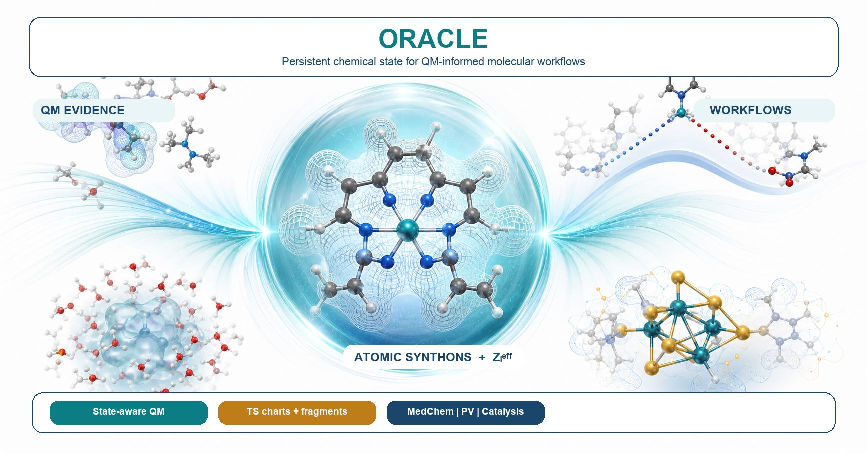
\includegraphics[width=\linewidth]{figures/oracle_theory_workflow_crossover.pdf}
\caption{Persistent chemical state connecting quantum-mechanical evidence with molecular workflows.}
\label{fig:oracle-theory-workflow}
\end{figure*}

\begin{figure*}[htbp]
\centering
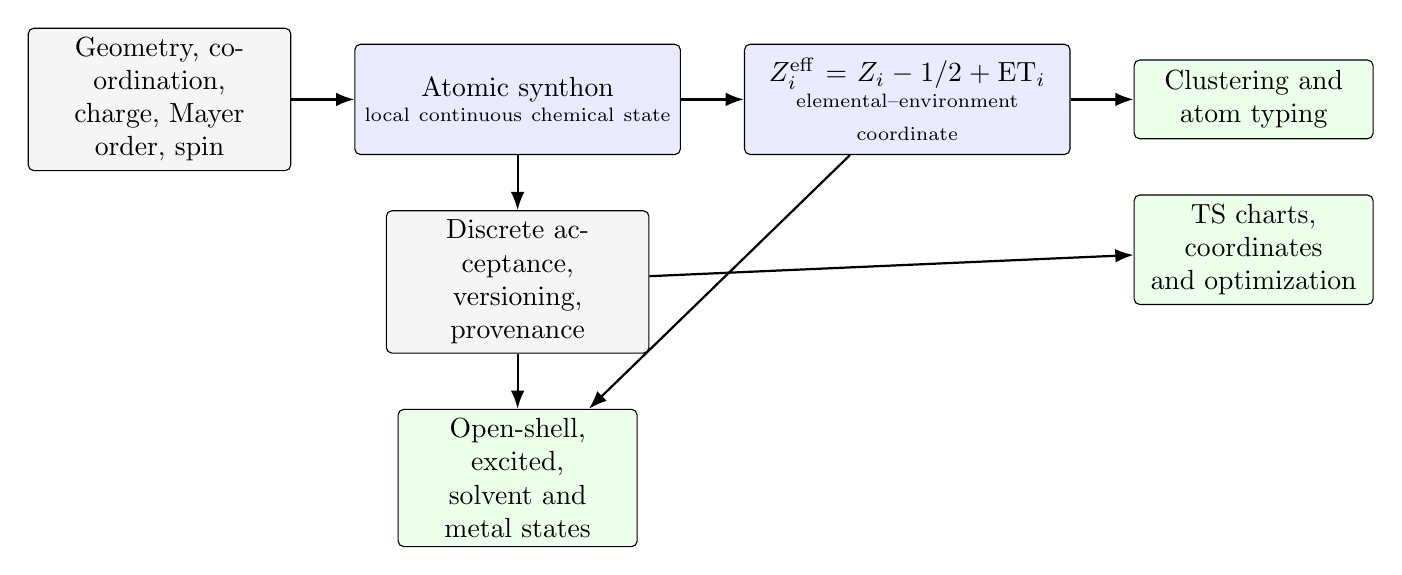
\begin{tikzpicture}[>=Latex, node distance=7mm and 8mm,
  box/.style={draw, rounded corners=2pt, align=center, minimum height=11mm,
    text width=31mm, fill=gray!8},
  core/.style={draw, rounded corners=2pt, align=center, minimum height=14mm,
    text width=39mm, fill=blue!8},
  app/.style={draw, rounded corners=2pt, align=center, minimum height=10mm,
    text width=28mm, fill=green!8}, arr/.style={->, thick}]
\node[box] (evidence) {Geometry, coordination,\\charge, Mayer order, spin};
\node[core, right=of evidence] (synthon) {Atomic synthon\\[-1mm]\scriptsize local continuous chemical state};
\node[core, right=of synthon] (zeff) {$Z_i^{\mathrm{eff}}=Z_i-1/2+\mathrm{ET}_i$\\[-1mm]\scriptsize elemental--environment coordinate};
\node[box, below=of synthon] (accept) {Discrete acceptance,\\versioning, provenance};
\node[app, right=of zeff] (cluster) {Clustering and\\atom typing};
\node[app, below=of cluster] (react) {TS charts, coordinates\\and optimization};
\node[app, below=of accept] (scope) {Open-shell, excited,\\solvent and metal states};
\draw[arr] (evidence) -- (synthon); \draw[arr] (synthon) -- (zeff);
\draw[arr] (zeff) -- (cluster); \draw[arr] (synthon) -- (accept);
\draw[arr] (accept) -- (react); \draw[arr] (accept) -- (scope);
\draw[arr] (zeff) -- (scope);
\end{tikzpicture}
\caption{Continuous chemical evidence organized into versioned molecular objects.}
\label{fig:chemical-module}
\end{figure*}

\section{Constructing an Executable Molecular State}

\subsection{The perception--calculation boundary}

From simplified molecular-input line-entry system (SMILES) or an enriched Cartesian/QCSchema record, the workflow builds an
inspectable molecular state with immutable snapshots.  \rev{Here
``immutable'' refers to a serialized snapshot: it is never edited in place.
A geometry, electronic result, accepted graph, or downstream structural
operation that changes a declared dependency creates a new state version with
a parent fingerprint; unchanged dependencies permit reuse of the previous
snapshot.  Thus ``perceived once'' means once per version, not once for all
future geometries, and ``persistent'' means persisted and reused until
targeted invalidation is triggered.}
(Figure~\ref{fig:architecture}).  Its primary chemical products are atom types
and local chemical descriptors (hereafter synthons);\cite{synthon_2024}
paired charges and bond orders; canonical rings and
aromaticity; exact symmetry operations and equivalence classes; hydrogen-bond
contacts; and alternative fragment views.  When requested, the same state
drives overlap reconstruction or an explicit geometry-optimization route.
Graphs, primitive coordinates and analytic Wilson matrices are generated
internally to support these products and remain available for audit.

Four layers remain distinct throughout the workflow: quantum-mechanical
evidence; the persistent molecular state that stores it; discrete objects
accepted from that evidence; and downstream operations that consume those
objects.  This separation makes it possible to update charges, bond orders,
spin or solvent metadata without silently replacing the molecular identity,
while allowing a changed dependency to trigger a controlled new state.

\begin{figure*}[htbp]
\centering
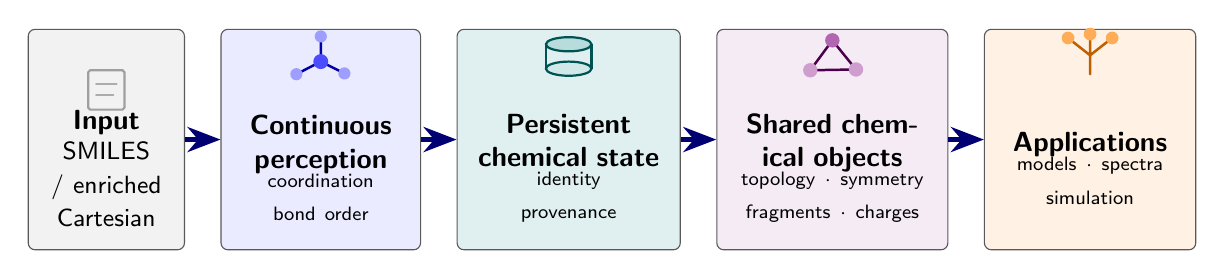
\begin{tikzpicture}[
  font=\sffamily,
  >=Latex,
  box/.style={draw=black!65,rounded corners=2.5pt,align=center,minimum height=2.80cm},
  input/.style={box,fill=gray!10,text width=1.75cm},
  evidence/.style={box,fill=blue!8,text width=2.30cm},
  state/.style={box,fill=teal!12,text width=2.60cm},
  objects/.style={box,fill=violet!8,text width=2.70cm},
  use/.style={box,fill=orange!10,text width=2.45cm},
  arrow/.style={-{Stealth[length=4.2mm,width=3.2mm]},line width=1.5pt,draw=blue!45!black}
]
\node[input] (in) {\rule{0pt}{0.62cm}\\[-2pt]\textbf{Input}\\[-1pt]\small SMILES / enriched Cartesian};
\node[evidence,right=0.45cm of in] (ev) {\rule{0pt}{0.62cm}\\[-2pt]
\textbf{Continuous\\perception}\\[-1pt]\scriptsize coordination\\bond order};
\node[state,right=0.45cm of ev] (st) {\rule{0pt}{0.62cm}\\[-2pt]
\textbf{Persistent\\chemical state}\\[-1pt]\scriptsize identity\\provenance};
\node[objects,right=0.45cm of st] (ob) {\rule{0pt}{0.62cm}\\[-2pt]
\textbf{Shared chemical objects}\\[-1pt]
\scriptsize topology $\cdot$ symmetry\\fragments $\cdot$ charges};
\node[use,right=0.45cm of ob] (use) {\rule{0pt}{0.62cm}\\[-2pt]
\textbf{Applications}\\[-1pt]\scriptsize models $\cdot$ spectra\\simulation};
\draw[arrow] (in)--(ev);
\draw[arrow] (ev)--(st);
\draw[arrow] (st)--(ob);
\draw[arrow] (ob)--(use);

% Compact vector pictograms keep the scientific flow readable at print size.
\begin{scope}[line cap=round,line join=round]
  % Input document.
  \draw[draw=gray!75,line width=0.8pt,rounded corners=0.7pt]
    ([xshift=-0.23cm,yshift=0.38cm]in.center) rectangle
    ([xshift=0.23cm,yshift=0.88cm]in.center);
  \draw[draw=gray!65,line width=0.7pt]
    ([xshift=-0.13cm,yshift=0.70cm]in.center) --
    ([xshift=0.13cm,yshift=0.70cm]in.center)
    ([xshift=-0.13cm,yshift=0.57cm]in.center) --
    ([xshift=0.09cm,yshift=0.57cm]in.center);

  % Continuous local network.
  \draw[draw=blue!65!black,line width=0.9pt]
    ([xshift=0cm,yshift=0.99cm]ev.center) --
    ([xshift=-0.31cm,yshift=0.83cm]ev.center)
    ([xshift=0cm,yshift=0.99cm]ev.center) --
    ([xshift=0.30cm,yshift=0.84cm]ev.center)
    ([xshift=0cm,yshift=0.99cm]ev.center) --
    ([xshift=0cm,yshift=1.31cm]ev.center);
  \fill[blue!70] ([yshift=0.99cm]ev.center) circle (2.7pt);
  \fill[blue!38] ([xshift=-0.31cm,yshift=0.83cm]ev.center) circle (2.2pt);
  \fill[blue!38] ([xshift=0.30cm,yshift=0.84cm]ev.center) circle (2.2pt);
  \fill[blue!38] ([yshift=1.31cm]ev.center) circle (2.2pt);

  % Versioned state/database.
  \draw[draw=teal!65!black,fill=teal!28,line width=0.8pt]
    ([yshift=1.21cm]st.center) ellipse (0.29cm and 0.09cm);
  \draw[draw=teal!65!black,line width=0.8pt]
    ([xshift=-0.29cm,yshift=0.90cm]st.center) --
    ([xshift=-0.29cm,yshift=1.21cm]st.center)
    ([xshift=0.29cm,yshift=0.90cm]st.center) --
    ([xshift=0.29cm,yshift=1.21cm]st.center);
  \draw[draw=teal!65!black,fill=teal!18,line width=0.8pt]
    ([yshift=0.90cm]st.center) ellipse (0.29cm and 0.09cm);

  % Linked chemical objects.
  \draw[draw=violet!60!black,line width=0.9pt]
    ([xshift=-0.28cm,yshift=0.88cm]ob.center) --
    ([yshift=1.26cm]ob.center) --
    ([xshift=0.30cm,yshift=0.89cm]ob.center) --
    ([xshift=-0.28cm,yshift=0.88cm]ob.center);
  \fill[violet!60] ([yshift=1.26cm]ob.center) circle (2.6pt);
  \fill[violet!38] ([xshift=-0.28cm,yshift=0.88cm]ob.center) circle (2.6pt);
  \fill[violet!38] ([xshift=0.30cm,yshift=0.89cm]ob.center) circle (2.6pt);

  % One state branching to multiple applications.
  \draw[draw=orange!75!black,line width=0.9pt]
    ([yshift=0.83cm]use.center) -- ([yshift=1.07cm]use.center)
    ([yshift=1.07cm]use.center) -- ([xshift=-0.28cm,yshift=1.29cm]use.center)
    ([yshift=1.07cm]use.center) -- ([yshift=1.34cm]use.center)
    ([yshift=1.07cm]use.center) -- ([xshift=0.28cm,yshift=1.29cm]use.center);
  \fill[orange!65] ([xshift=-0.28cm,yshift=1.29cm]use.center) circle (2.3pt);
  \fill[orange!65] ([yshift=1.34cm]use.center) circle (2.3pt);
  \fill[orange!65] ([xshift=0.28cm,yshift=1.29cm]use.center) circle (2.3pt);
\end{scope}
\end{tikzpicture}
\caption{A persistent perceived state shared by downstream applications.}
\label{fig:architecture}
\end{figure*}

Black-box operation combines automatic selection of ring algorithms, symmetry
frames, fragment overlaps, electronic-population analysis and numerical
backends with inspectable evidence and provenance.  Applications transform
the stored state through explicit, versioned updates.

For clarity, the terminology follows three levels.  \emph{Continuous
evidence} denotes coordination, charge, bond order and the derived local
descriptors.  The \emph{persistent state} contains the exact graph, rings,
symmetry, atom classes and fragments accepted from that evidence.  Named
service programs are defined together in the Computational Details.  They
supply input operations and electronic observables without changing this
chemical hierarchy.

\subsection{Continuous evidence and discrete chemical objects}

The descriptor construction follows three chemically intuitive questions.
First, how many neighboring atoms influence a center, and with what smoothly
varying strength?  Second, how are charge and bond order distributed through
that environment?  Third, which local environments remain equivalent when
geometry, coordination or electronic populations change slightly?  The
continuous coordination number answers the first question with a smooth
neighbor count.  The atomic synthon gathers the geometric and electronic
answers into a local descriptor, while the effective atomic number provides a
single continuous coordinate for comparing related environments.  These
quantities connect smoothly varying chemical evidence to elemental identity
and the accepted exact graph.

The continuous coordination number (CNA) illustrates the evidential layer,
\begin{equation}
\mathrm{CNA}_i=\sum_{j\ne i}\frac{1}{2}
\left[1+\operatorname{erf}\!\left(
\alpha_{\mathrm{CNA}}(R^0_{ij}-R_{ij})\right)\right],
\end{equation}
with coordination-dependent covalent radii obtained by smooth Hermite
interpolation of Pyykk\"o data.\cite{pyykko_radii_2009}  The resulting
connectivity weight supplies topological evidence; the stored chemical bond
order remains the single value used by downstream models.

To prevent a similar ambiguity in the electronic description, the state stores
one charge and one bond order at a single, internally consistent availability
level.  Complete Charge Model 5 (CM5) charges and Mayer bond orders define the
quantum-mechanical (QM) level for the whole structure;
\cite{cm5_2012,mayer_bond_order_1983} otherwise the state adopts the paired
electronegativity/Pauling geometry estimate.  The selected bond order is
resolved continuously into non-negative $\sigma$, $\pi$ and $\pi\pi$
components whose sum recovers the original value.

The local descriptors used in this workflow are defined as follows.  With
$\mathcal N(i)$ the continuously perceived neighbors,
$\widetilde R^{\mathrm{cov}}$ the coordination-adjusted covalent radius and
$\bar R_i$ the mean incident distance, the compactness and radial-dispersion
components are
\begin{align}
C_i&=\frac{1}{|\mathcal N(i)|}\sum_{j\in\mathcal N(i)}
\frac{\widetilde R_i^{\mathrm{cov}}+\widetilde R_j^{\mathrm{cov}}}
{R_{ij}+\widetilde R_i^{\mathrm{cov}}+\widetilde R_j^{\mathrm{cov}}},\\
D_i&=\frac{1}{|\mathcal N(i)|\bar R_i}
\sum_{j\in\mathcal N(i)}|R_{ij}-\bar R_i|.
\end{align}

The third geometric component measures angular strain and extends the same
description beyond ordinary organic valence.  The method forms a continuous
electronic-domain (ED) count $N_i^{\mathrm{ED}}$ from coordination, lone-pair and
open-shell domains and evaluates
\begin{equation}
S_i=\left[
\frac{1}{\binom{N_i^{\mathrm{ED}}}{2}}
\sum_{j<k}\left(
\cos\theta_{ijk}-\cos\bar\theta(N_i^{\mathrm{ED}})
\right)^2
\right]^{1/2}.
\label{eq:synthon-angular}
\end{equation}
The reference mean angles for domain counts 2, 3, 4, 5, 6, 8 and 12 are
$180.0^\circ$, $120.0^\circ$, $109.47^\circ$, $120.0^\circ$,
$90.0^\circ$, $90.0^\circ$ and $63.43^\circ$, respectively, with smooth
Hermite interpolation between integer counts.  Equation~
\ref{eq:synthon-angular} therefore treats tetrahedral, hypervalent and
high-coordinate environments within one expression.

These components, the atomic charge and the incident bond-order sums define
the seven-component atomic synthon
\begin{equation}
\mathbf{s}_i=(q_i,C_i,D_i,S_i,
I_i^{(\sigma)},I_i^{(\pi)},I_i^{(\pi\pi)}),
\label{eq:synthon}
\end{equation}
where
$I_i^{(x)}=\sum_{j\in\mathcal N(i)}\mathrm{BO}_{ij}^{(x)}$,
$x\in\{\sigma,\pi,\pi\pi\}$, collects each non-negative incident bond-order
component.  These definitions remain continuous in geometry, coordination
and bond order.

Higher-order synthons are built compositionally:
\begin{align}
\mathcal S_{ij}^{(\mathrm{bond})}
  &=\left(\mathbf s_i,\mathbf s_j,\mathrm{BO}_{ij}\right),\\
\mathcal S_{ijk}^{(\mathrm{angle})}
  &=\left(\mathcal S_{ij}^{(\mathrm{bond})},
           \mathcal S_{jk}^{(\mathrm{bond})},\cos\theta_{ijk}\right),\\
\mathcal S_{ijkl}^{(\mathrm{dihedral})}
  &=\left(\mathcal S_{ijk}^{(\mathrm{angle})},
           \mathcal S_{jkl}^{(\mathrm{angle})},
           \cos\phi_{ijkl},\cos^2\phi_{ijkl}\right).
\end{align}
Ring synthons collect the ordered bond and angle descriptors of a canonical
cycle; hydrogen-bond synthons add the donor--hydrogen--acceptor descriptors
and continuous contact geometry.  The same effective-atomic-number coordinate
combines elemental identity with the local environment.  Complete
normalizations and similarity metrics
are given in the Supporting Information.

Atomic types are obtained by element-preserving complete-link clustering of
the atomic synthons, with every accepted class retaining its centroid,
maximum descriptor spread and generating thresholds.  To connect this native
description with an established force-field vocabulary, the workflow also
translates the accepted graph, aromatic annotation and bond-order components
into General Amber Force Field, version~2 (GAFF2), labels.\cite{gaff_2004}
For saccharin, this maps aromatic carbon, carbonyl carbon, sulfur-bound oxygen,
amide nitrogen and hypervalent sulfur to \texttt{ca}, \texttt{c}, \texttt{o5},
\texttt{n} and \texttt{s6}, respectively; the carbonyl oxygen is represented by
the distinct \texttt{o} class.  The
versioned mapping leaves the continuous native type unchanged and records
mapping coverage explicitly; complete rules, including phosphorus and sulfur,
are given in the Supporting Information.

Synthon-derived classes preserve continuous chemical similarity for
equivalence, fragment transfer and model construction.  GAFF2 labels connect
the same perceived state to an established force-field vocabulary.  The
saccharin labels below document this interoperable path while every
perception decision remains anchored to the underlying continuous evidence.

Equation~\ref{eq:synthon} and its weighted sums admit unrestricted
coordination and therefore avoid the tetravalence ceiling implicit in many
organic-chemistry typing schemes.  The same representation consequently
describes conventional organic environments and highly coordinated centers.
In fixed FeF$_n$
coordination spheres with $n=4,6,8,10,$ and 12, the accepted central degrees
are exactly $n$ and the corresponding continuous coordination numbers are
3.99, 5.98, 7.97, 9.97, and 11.96.  Radial expansion of the 12-coordinate
sphere gives a smooth decay from approximately 12 to zero across a single
coordination-independent expression.  The perception layer and its
covalent-radius support span elements 1--118.  Quantitative electronic
descriptors use a complete internally generated or user-supplied
charge/bond-order pair.

Continuous evidence leads to exact topology.  Once a covalent
graph has been accepted, deterministic Horton candidates, recursive chord
splitting and binary independence selection produce a canonical minimum-length cycle basis
of rank $|E|-|V|+c$.\cite{Horton1987,ring_perception_2000,ring_path_2009}
Each cycle is serialized as an ordered canonical atom sequence.  Ring systems,
atom--ring and bond--ring incidence, and label-preserving automorphisms are
then exact objects.  Aromaticity is stored separately as a conservative
annotation accepted from continuous delocalization evidence together with
the local graph and electronic environment.

Hydrogen bonds make this continuous--discrete distinction especially clear.
Smooth distance and angular terms, referenced to van der Waals radii, quantify
the evidence for a donor--H$\cdots$acceptor contact,\cite{uff_1992} while an
accepted contact remains distinct from the covalent edge set.  An
intramolecular contact may therefore close a pseudocycle through the covalent
path, whereas an intermolecular contact joins otherwise separate covalent
components only at the interaction resolution.  The current implementation
recognizes chemically compatible nitrogen, oxygen, phosphorus and sulfur
sites, and the quantitative response library described below extends the
parent hydride environments with systematically substituted monomer/dimer
combinations.

A distinct, geometry-certified shared-hydrogen motif is
resolved before the ordinary one-neighbor hydrogen constraint is enforced.
For each hydrogen, candidate B, N, O, P, and S neighbors must lie within the
sum of the corresponding covalent radii plus 0.60~\AA.  The two nearest
candidates are accepted only when their distances agree within 0.15~\AA{} or
10\%, and when the heavy-atom--H--heavy-atom angle is at least
\(140^\circ\) for N/O/P/S bridges or \(60^\circ\) for a
boron-containing three-center bridge.  A certified hydrogen is then allowed
exactly the two detected neighbors; every other hydrogen remains monovalent.
The two contacts enter the persistent graph, cycle inventory, and provenance
together, which covers symmetric proton-transfer structures and B--H--B
bridges without molecule-specific templates.

\subsection{Electronic closure at the L0 level}

To close the perceived state at the level required by its electronic
descriptors, the workflow first retains any complete, provenance-bearing set of
charges and bond orders supplied by the user.  When such data are absent, it
generates them with the new L0 baseline: a gas-phase calculation using the
parameter-free Perdew--Burke--Ernzerhof hybrid with 25\% exact exchange (PBE0)
and the Karlsruhe valence triple-zeta basis with polarization
(def2-TZVP).\cite{pbe0_1999,def2_2005}  This parameter-free combination
provides a consistent operational baseline for populations and structures over
the element range supported by the corresponding all-electron bases and
effective-core potentials.

The calculation is performed through an \emph{internal} in-memory interface to
the Python-based Simulations of Chemistry Framework (PySCF), which supplies
Complete Charge Model 5 (CM5) charges and Mayer bond orders from the same
electronic state.\cite{pyscf_2018,cm5_2012,mayer_bond_order_1983} Calculations use tight
self-consistent-field convergence and the native scalar-relativistic def2
effective-core potentials from rubidium through radon, which define the
current L0 electronic domain.  Complete electronic arrays select L0;
otherwise the paired electronegativity/Pauling estimate applies to the whole
object.  Settings and inputs are reported in the Supporting Information.  L0
is a single fixed-geometry closure; for larger molecules its overlapping-core
and halo construction distributes the QM work across connected fragments.

For a large molecule, the same electronic closure is obtained from overlapping
local calculations.  Every atom belongs to exactly one fragment core, every
perceived covalent pair occurs in at least one L0 core-plus-halo fragment, and
the fragments together form a connected overlap graph.  Core observations
reconstruct the molecular charges, while repeated halo observations quantify
their sensitivity to the artificial fragment boundary.  Once these local
values have been assembled, the unique minimum-weight displacement restores
the molecular charge,
\begin{equation}
 q_i=q_i^{\mathrm{raw}}-
 \frac{Q_{\mathrm{raw}}-Q_{\mathrm{mol}}}
 {w_i\sum_jw_j^{-1}}.
\label{eq:l0-charge-assembly}
\end{equation}
Mayer values come from the fragment in which each pair lies deepest, averaging
only observations of equal interior rank.  Overlap dispersion remains an
atomwise boundary diagnostic.  Core, bond, overlap-graph and electronic-level
completeness are verified before assembly; neutral electrostatic groups for
fast-multipole evaluation are constructed afterward.  The default two-bond
halo expands whenever a boundary would cut a conjugated, ring,
metal-coordination or otherwise protected environment.

The frozen Gly--Ala--Gly audit gives a concrete large-state example: three
core-plus-two-shell fragments cover all 27 atoms and all 26 covalent bonds,
with one PBE0/def2-TZVP single point per fragment.  Relative to the direct
full-molecule calculation, the assembled CM5 vector has a root-mean-square (RMS) error of
0.0032~$e$ and a maximum error of 0.0101~$e$; the complete ownership map and
boundary diagnostics are archived in the Supporting Information.  This
establishes the intended overlap reconstruction route for the electronic
closure and provides a molecular-scale accuracy benchmark for fragment
assembly.

\subsection{Quantum observables as state updates}

The perceived state and the quantum calculation form a bidirectional feedback
loop.  An initial geometry is first perceived from SMILES or
Cartesian coordinates.  A single L0 calculation at that guess supplies CM5
charges and the total Mayer matrix.  For an unrestricted state it additionally
supplies the signed spin-selective Mayer matrix
\begin{equation}
B_{AB}^{\alpha-\beta} =
2\sum_{\mu\in A}\sum_{\nu\in B}
\left[
(P^\alpha S)_{\mu\nu}(P^\alpha S)_{\nu\mu}
-
(P^\beta S)_{\mu\nu}(P^\beta S)_{\nu\mu}
\right],
\label{eq:spin-mayer}
\end{equation}
in the same atomic-orbital partition used for the total Mayer order.
$B_{AB}^{\alpha-\beta}$ vanishes for a restricted closed shell and changes
sign when the spin labels are exchanged.  It measures spin-selective
covalency on a bond and complements the atomwise Hirshfeld
$\alpha-\beta$ population.

The CM5 vector updates electrostatic environments, the total Mayer matrix
updates bond-order components and aromatic conjugation, and the
$\alpha-\beta$ quantities identify where an open-shell guess carries its
spin.  These observables are attached to the persistent state and used to
regenerate or refine the geometry with the same accepted topology.  The
refined structure is then perceived again; only after topology, charge,
aromaticity and spin audits pass does the production electronic-structure
calculation start.  Thus the operational sequence is
\[
\begin{aligned}
\text{guess}&\longrightarrow\text{perception}
\longrightarrow\text{L0 CM5/Mayer}
\longrightarrow\text{geometry update}\\
&\longrightarrow\text{re-perception}
\longrightarrow\text{production QM}.
\end{aligned}
\]
Because the total and spin-selective Mayer maps vary continuously, modest
geometrical changes update this loop without forcing a premature change of
chemical identity.

Hydrogen bonding is then separated from the intrinsic monomer charge while
covalent identity remains fixed.  The construction is formulated as a fluctuation
about a CM5 population evaluated at a declared reference geometry
$\mathbf R_{\mathrm{ref}}$.  For every accepted
D--H$\cdots$A contact $c$, the dimer library supplies a unit response vector
$\Delta\mathbf q_c$, including separately donor polarization, acceptor
polarization and charge transfer.  If the reference geometry already contains
hydrogen bonds, its CM5 values include those effects.  The hydrogen-bond-free
baseline is recovered by
\begin{equation}
q_i^0=q_i^{\mathrm{CM5}}(\mathbf R_{\mathrm{ref}})
-\sum_c s_c(\mathbf R_{\mathrm{ref}})\Delta q_{i,c}.
\label{eq:hbond-intrinsic-reference}
\end{equation}
At an arbitrary geometry,
\begin{equation}
q_i(\mathbf R)=q_i^{\mathrm{CM5}}(\mathbf R_{\mathrm{ref}})
+\sum_c\left[s_c(\mathbf R)-s_c(\mathbf R_{\mathrm{ref}})\right]
\Delta q_{i,c}.
\label{eq:hbond-charge-response}
\end{equation}
Equation~\ref{eq:hbond-charge-response} reproduces the input CM5 charges at
$\mathbf R_{\mathrm{ref}}$ and tends continuously to $q_i^0$ as the relevant
contacts dissociate.  A zero-contact reference gives
$q_i^0=q_i^{\mathrm{CM5}}$.

The reference CM5 vector already contains the electronic response of its
molecular environment.  Additional polarization and charge transfer are
assigned to recognized events, beginning with hydrogen-bond formation.
Changes in coordination, bond order, ion pairing, metal--ligand contacts,
ring closure or local descriptors can identify further candidates; quantitative
response is activated only when represented in the resident library.

Donor and acceptor polarization are separately fragment neutral; the
charge-transfer vector is neutral only over the complete complex.  The
response is confined to the active X--H bond and, where present, the local
C=O or N--C=O conjugated unit.  Van der Waals radii determine its radial
amplitude:
\begin{equation}
s_{\mathrm{HB}}(r)=
\frac{\exp[-r/(R_{\mathrm{vdW},H}+R_{\mathrm{vdW},A})]}
{\exp[-r_{\mathrm{ref}}/(R_{\mathrm{vdW},H}+R_{\mathrm{vdW},A})]}.
\label{eq:hbond-charge-switch}
\end{equation}
The correction vanishes outside the selected contact domain, where
$q_i$ smoothly returns to $q_i^0$.  Within that domain, the resident table
retains the chemically transparent $4\times5$ product of four donor classes
(O--H, N--H, P--H and S--H) and five acceptor classes (O, N, carbonyl O, P and
S).  The table averages 320 rigid PBE0/def2-TZVP dimers.  Four distinct donor
environments and four distinct acceptor environments are crossed within each
of the 20 donor--acceptor classes, giving 16 chemically audited observations
per executable rule.  The substituted series spans alcohols, amines,
carbonyl compounds, phosphines and thiols while preserving the same
fixed-geometry protocol.

The averaging preserves the physical decomposition by treating charge
transfer, donor-local polarization and acceptor-local polarization
separately, after which the canonical neutral atomwise vectors are rescaled to
the corresponding mean displaced charges.  Across the table, mean Mayer
H$\cdots$A orders range from 0.031 to 0.109 and mean charge-transfer
magnitudes from 0.011 to 0.078~$e$.  The within-class sample standard
deviations are 0.0018--0.014~$e$ for donor polarization,
0.002--0.008~$e$ for acceptor polarization and 0.005--0.017~$e$ for
charge transfer.  This spread is chemically informative: it measures the
effect of substitution within a donor--acceptor class and is retained in the
table alongside the uncertainty in its mean.  Figure~\ref{fig:hbond-parameter-map} shows the
means and their bootstrap uncertainty, while the Supporting Information table
also reports the sample dispersion and provides the individual observations,
bootstrap 95\% confidence intervals,
leave-one-environment-out sensitivities and signed vectors.  Across all
response components, the largest absolute bootstrap half-width and
leave-one-environment-out shift are 0.008 and 0.009~$e$, respectively.
Thus the balanced factorial design resolves real environmental dispersion
while keeping the executable class means stable on the absolute charge scale.
The resulting class means are stable at the resolution supported by this
factorial design and are available as executable parameters for constructing
hydrogen-bond-adjusted charges from CM5 populations.

Water uses the noniterative
missing-coordination and charge-transfer model introduced in
Equations~18--20 of Ref.~\citenum{barone2022gfq}, replacing its integer
hydrogen-bond counts by the continuous contact strength and its isolated-water
reference by the symmetry-projected L0 CM5 vector
$(-0.674,+0.337,+0.337)~e$.  This is the water specialization of
Equations~\ref{eq:hbond-intrinsic-reference} and
\ref{eq:hbond-charge-response}.  The published condensed endpoint is the
ForceBalance-refined three-point transferable intermolecular potential
(TIP3P-FB) vector $(-0.848,+0.424,+0.424)~e$, and the published
water--water transfer scale is $\beta=0.10~e$.  The two donor and two acceptor
capacities share the CM5-to-TIP3P-FB polarization increment symmetrically.
Consequently, isolated water is exactly CM5, whereas the central molecule of
the symmetric pentamer, which donates and accepts two hydrogen bonds, is
exactly TIP3P-FB and exactly neutral.  The two donated and two accepted
charge-transfer contributions cancel at that endpoint.

The $4\times5$ table is a versioned runtime resource of the common chemistry
layer and a directly executable product of the validation.  A single shared
application programming interface (API) accepts connectivity, geometry and either intrinsic or
environment-polarized CM5 charges, then returns tuned charges together with
separate polarization, charge-transfer and contact diagnostics.  Repeated
optimization, exploration and simulation steps reuse the same
recognition plan and persistent skinned pair list.  At a nonperiodic boundary,
the same closed-form rule supplies the missing neutral polarization.  The
published water specialization and the general dimer-derived CM5 extension
remain distinct, auditable and available throughout the workflow.
The corresponding electrostatic construction is illustrated in
Figure~\ref{fig:l0-electrostatics}.

\begin{figure*}[htbp]
\centering
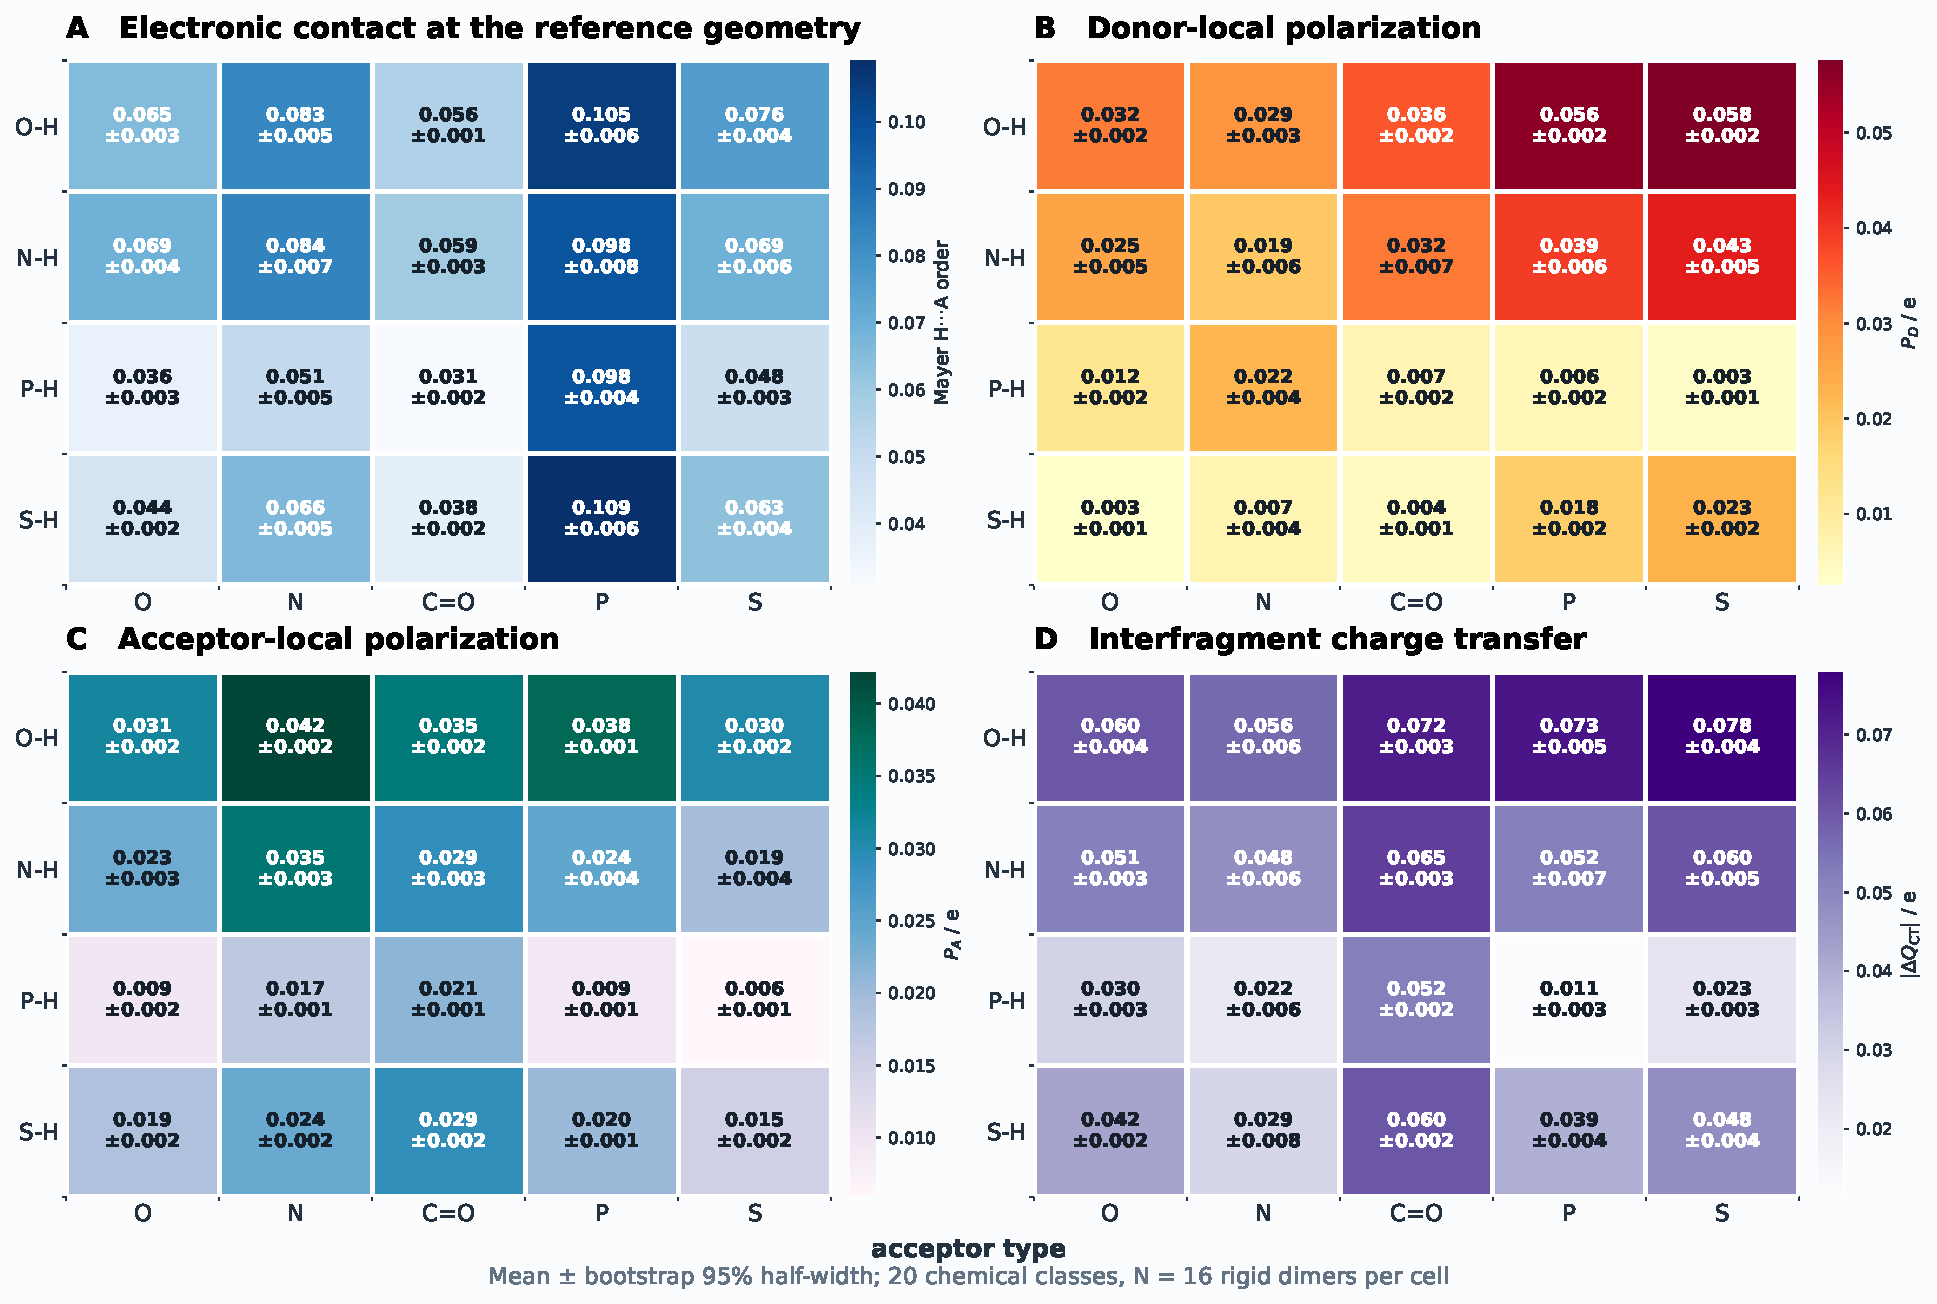
\includegraphics[width=\linewidth]{figures/oracle_hbond_parameter_map.pdf}
\caption{Mean hydrogen-bond responses across 20 donor--acceptor classes. Panels (a)--(d) show electronic contact, donor-local polarization, acceptor-local polarization, and interfragment charge transfer.}
\label{fig:hbond-parameter-map}
\end{figure*}

\begin{figure*}[htbp]
\centering
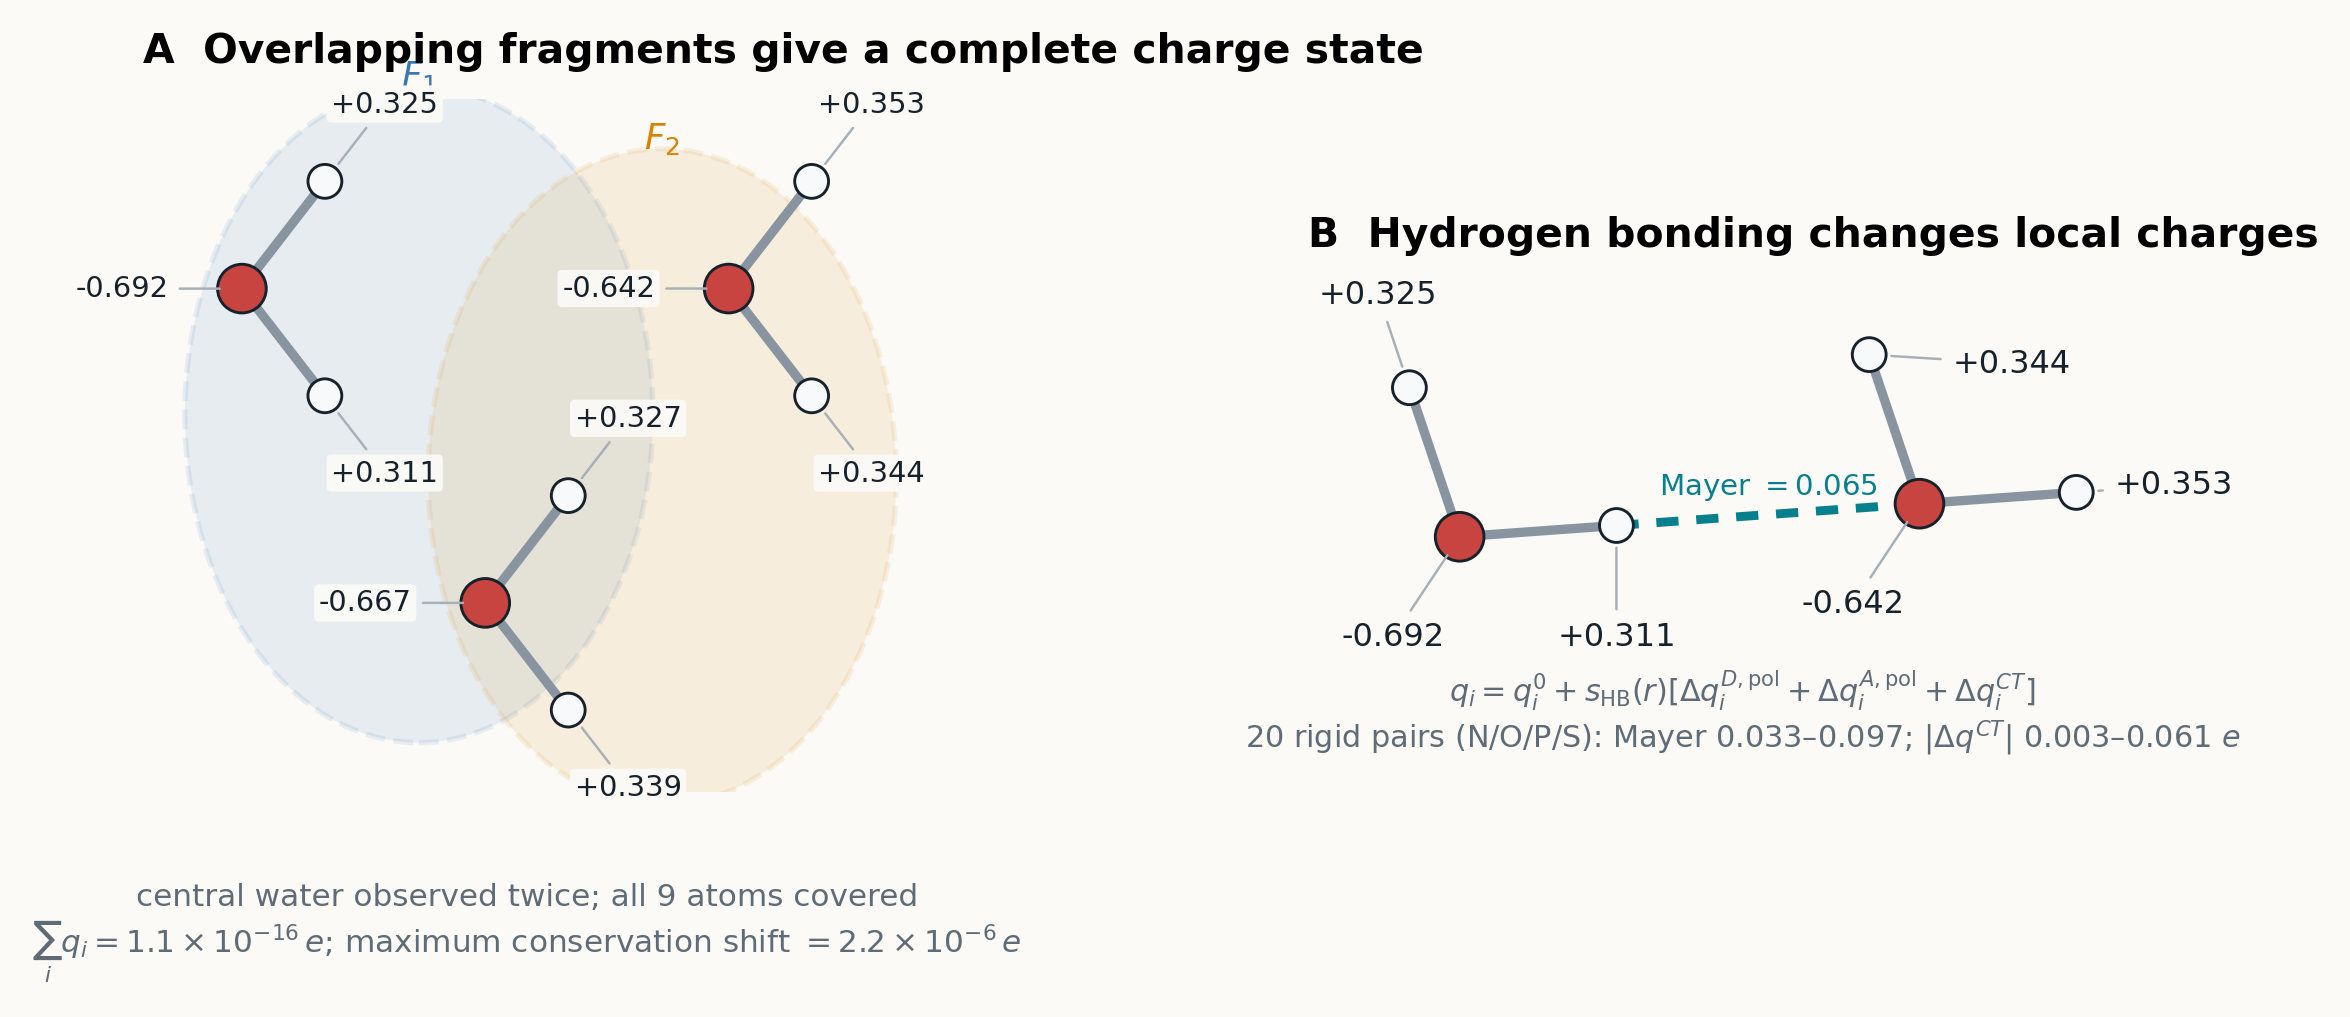
\includegraphics[width=\linewidth]{figures/oracle_l0_electrostatics.png}
\caption{Baseline electrostatic closure from charge assembly and local hydrogen-bond response. Panels (A)--(B) show charge completion by overlapping fragments and the local response to hydrogen bonding.}
\label{fig:l0-electrostatics}
\end{figure*}

\subsection{Geometry and population decision path}

For conventional organic systems, the practical objective is a reproducible
path from a SMILES string to an accurate geometry.  Transition-metal systems
start from the enriched Cartesian state defined above or from a coordination
specification that first generates candidate Cartesian structures.  Only three level labels are needed for this optional
route.  Beyond these three active labels, two additional archival or reserved
identifiers appear in file names and figures.  The baseline introduced here
(L0) is PBE0/def2-TZVP; a higher-level
geometry (L1) is obtained with a double-hybrid method and an extended basis set, and PL1
applies a further posterior correction to covalent bond lengths and
hydrogen-bond geometries.  These levels retain the definitions established in
the structural-accuracy ladder and its underlying high-level, templating and
posterior-correction developments.
\cite{acr_2026,external_MRCC_2025,PCS141_2024,synthon_2024,DPCS3_2023}
When the full route is requested, the workflow proceeds incrementally,
\begin{equation}
\text{molecular input}\longrightarrow
\text{initial Cartesian structure}\longrightarrow
\mathrm{L0}\longrightarrow\mathrm{L1}\longrightarrow\mathrm{PL1},
\label{eq:geometry-ladder}
\end{equation}
reusing the approximate curvature accumulated by each optimization to
initialize the next.  If a Cartesian file is supplied, its geometry is
preserved unless optimization is explicitly requested, in which case the same
ladder starts from that structure.

Population analysis and geometry optimization remain independent requests.
Accordingly, the water, hydrogen-bond, ferrocene and cisplatin calculations
reported here are fixed-geometry single points.  When a larger target is
requested, compatible fragments from the published 2025 building-block
library and its 2026 extension are reused whenever possible; otherwise,
connected overlapping fragments are generated until every atom and covalent
pair has been defined.  The Supporting Information gives the corresponding
input details, the reuse of Hessian information between stages and the
complete decision tree.

\rev{L0 is an electronic closure and feedback route that complements
geometry-only perception.  Geometry-only calls accept a complete state or
request topology, rings, symmetry and continuous geometric descriptors.  L0
supplies the reproducible CM5/Mayer/spin observables used by the feedback
examples.  Functional and basis sensitivity, together with the geometry-only
baseline, define the next expansion of the electronic benchmark.}

\rev{The current ORACLE implementation also supports an explicitly requested
single-geometry transition-state perception.  Weak acyclic contacts that may
represent breaking interactions and near-covalent contacts that may represent
forming interactions are retained as typed transition-state evidence, but are
not silently promoted to the constitutional graph.  The TS contract records
the reactive kernel, the allowed chart policy (reactive distance or prescribed
pseudobond), the reactive zones, and the provenance of every decision.  When
several admissible primitive combinations describe the same reactive zone, the
candidate charts are compared through the normalized condition number of their
Wilson-$B$ representation.  Provided the declared conditioning trigger and
minimum relative-gain gate are satisfied, ORACLE selects the candidate with
the lowest condition number and records the comparison and selection.  Thus a
formally complete chart is not accepted merely because it has full rank: among
valid alternatives, numerical conditioning is an explicit chemical-workflow
criterion.}

The examples below illustrate this feature through representative
transition-state geometries with insertion, ring-opening, dissociation,
torsional-isomerization and rearrangement topologies, including two
rank-24 bicyclobutane structures (Figure~\ref{fig:baker-ts-examples}).

\begin{figure*}[htbp]
\centering
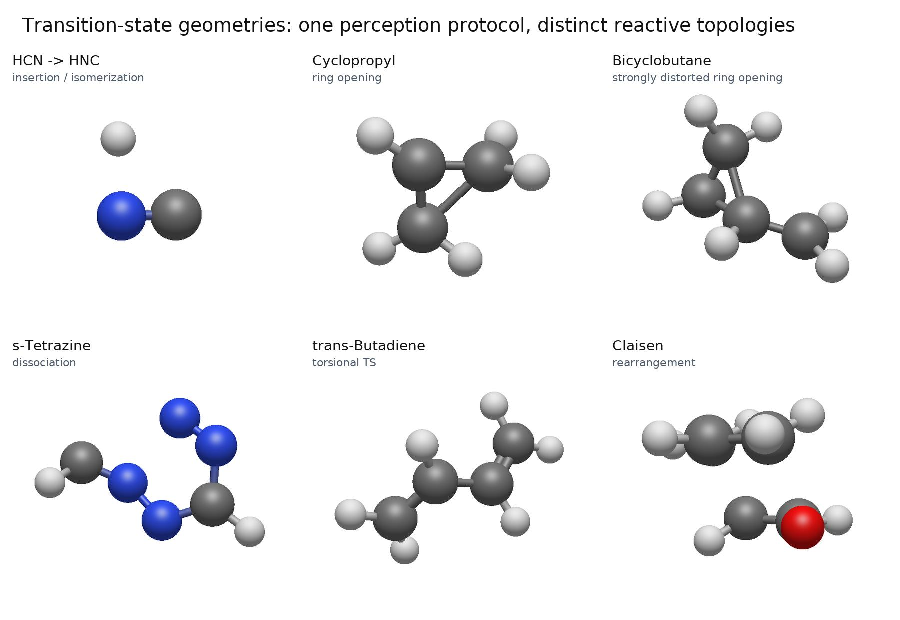
\includegraphics[width=0.96\linewidth]{figures/oracle_baker_ts_examples.pdf}
\caption{Transition-state geometries spanning distinct reactive topologies.}
\label{fig:baker-ts-examples}
\end{figure*}

\subsection{Executable symmetry}

Symmetry becomes executable by storing each accepted operation as
\begin{equation}
g=(\mathbf R_g,\pi_g),
\qquad
\mathbf R_g^\mathsf T\mathbf R_g=\mathbf 1,
\qquad
\det\mathbf R_g=\pm1,
\end{equation}
where $\pi_g$ is the element-preserving atom permutation induced by
$\mathbf R_g$.  Identity, closure, inverse, matrix--permutation composition
and mapping residuals are verified jointly.  The complete action can therefore
be applied directly to atoms, polar vectors, axial vectors or primitive
coordinates.

Degenerate inertia tensors receive a deterministic, rigidly covariant
treatment.  For a symmetric top, the unique principal axis is fixed by the
inertia tensor and the free perpendicular plane is anchored to an actual
point-set operation: either a perpendicular twofold axis or the normal to a
vertical mirror plane.  Spherical tops instead recover the complete point-set
isometry from element- and metric-compatible triples.  Accepted matrices are
conjugated back to the input Cartesian frame before serialization, so neither
the group nor its atom action depends on an arbitrary eigensolver basis.

Finite groups are required to have their exact order and to close jointly in
matrix and permutation space.  This gate covers the low-order groups
$C_1$, $C_s$ and $C_i$; the complete supported axial families
$C_n$, $C_{nv}$, $C_{nh}$, $D_n$, $D_{nh}$ and $D_{nd}$; the pure improper
families $S_{2n}$; and the polyhedral families $T$, $T_d$, $T_h$, $O$, $O_h$,
$I$ and $I_h$.  Linear molecules are treated separately as $C_{\infty v}$ or
$D_{\infty h}$ and are not subjected to an artificial finite-group closure.

The serialized operation--permutation pairs are also the sole molecular
symmetry authority passed to coordinate construction.  ORACLE uses the same operation
classification, and character construction uses the stored matrices whenever
a label alone is insufficient.  The workflow can therefore build every irreducible
representation and its symmetry-adapted linear combinations (SALCs) from the
complete ORACLE action, within homogeneous coordinate families and without
selecting a convenient subgroup or reconstructing symmetry independently.

Quasi-symmetry uses an absolute Cartesian threshold $\tau$, a stable-threshold
plateau and an explicit residual margin.  If a complete group $G$ is accepted,
the geometry may be projected by
\begin{equation}
\mathbf r_i^{\mathrm{sym}}=\frac{1}{|G|}
\sum_{g\in G}\mathbf R_g^\mathsf T\mathbf r_{\pi_g(i)}.
\end{equation}
The threshold, operation residuals and required Cartesian displacement remain
part of the state.  Symmetry projection follows acceptance of the complete
group under the declared threshold.

\rev{Projection is a coordinate transformation with a recorded displacement.  The quasi-$O_h$
cubane audit gives a maximum displacement of $3.3\times10^{-4}$~\AA{} and reanalysis
restores the 48 operations to a residual below $10^{-15}$~\AA{}.  Frequencies,
Derivative properties are evaluated on the projected geometry whenever the
recorded displacement is chemically relevant.}

\subsubsection{Assignment and adjustment of almost symmetric structures}

Assignment tests whether the observed point set supports a complete finite
group within a declared absolute tolerance.  Adjustment applies the
group-average projector only after every operation has a compatible atom
permutation and the set has the expected order.  An incomplete group would
destroy the projector property; the diagnostic is recorded and the structure
is left unchanged.

This separation is essential for experimental, edited, force-field and
unconstrained optimized geometries, which often retain symmetry only
approximately.  Water and formaldehyde regressions identify stable tolerance
plateaus, store the complete $C_{2v}$ permutations, project, and reanalyze the
adjusted structures.  The output records both the assigned symmetry and the
Cartesian change required to make it exact.

Exact molecular symmetry is complemented by local regularity because
medium-to-large molecules are often globally $C_1$ while a coordination sphere, substituted
ring or repeated fragment remains approximately symmetric.  Continuous
elemental, radial and local-environment descriptors order these
domains and define reproducible local equivalence classes.  The stored
molecular group provides global equivalence.

For applications that change geometry, the workflow internally generates ordered
primitive coordinates and their analytic Wilson matrix from the frozen state.
They support reconstruction and correction internally; their definitions and
rank tests are given in the Supporting Information.

\subsection{Persistent aromaticity and differential structural correction}

Aromaticity is stored as more than an atom flag.  For each accepted ring,
the state records the contributing atoms and bonds, plane deviations, electron
count when available, and the decision criterion: $4n+2$, a fused conjugated
component, or a metal-coordinated $\eta^5$ cycle.  Local $p$-orbital eligibility
includes common group-13, -14, -15, and -16 centers.  During structural
correction, every stored aromatic ring supplies a local best-fit-plane
projector, with proposals for shared atoms averaged consistently.  A helically arranged fused
system therefore retains distinct local ring planes throughout projection.

Given a target geometry calculated at level $L$ and a matched accurate
fragment $f$, the correction transfers each supported primitive as
\begin{equation}
q_\alpha^{\mathrm{corr}}(M;L)=q_\alpha(M;L)+
\left[q_\alpha(f;\mathrm{ref})-q_\alpha(f;L)\right].
\label{eq:differential}
\end{equation}
The molecule and every selected fragment use the same level $L$, so the
bracket isolates the method-specific error.
Equation~\ref{eq:differential} applies simultaneously to stretches, bends,
torsions and out-of-plane coordinates.  Environments outside the resident
library become explicit requests for targeted fragment calculations.
Back-transformation is
followed by the persistent aromatic and finite-group projectors and complete
reperception.

A local target displacement $\Delta\mathbf q_S$ is reconstructed by the
regularized update
\begin{equation}
\Delta\mathbf x=
\mathbf B_S^\mathsf T
\left(\mathbf B_S\mathbf B_S^\mathsf T+\lambda\mathbf I\right)^{-1}
\Delta\mathbf q_S.
\label{eq:backtransform}
\end{equation}
The examples below use this operation for core--valence, conjugation and
selected-pair corrections.  Structural correction consumes the
perceived state through a downstream model that supplies parameter
construction, validation, coordinate selection and force-field fitting.

\section{A Validation Designed Around State Transfer}

The validation mirrors the structure of the central claim.  It first tests
invariance to rigid motion and atom ordering, then verifies exact recovery of
topology, cycle rank, aromaticity, finite groups, primitive rank and
serialization, and finally examines reuse in chemically distinct applications
with explicit reference coverage.  Inputs, fingerprints, scripts and
machine-readable outputs are documented in the Supporting Information.  The reported tests
quantify reproducibility and internal consistency, while frozen inputs and
executable records make each contract independently testable.

As a secondary efficiency check, we performed a controlled handoff ablation on eight systems
spanning 3--176 atoms.  The full route supplied a validated ORACLE state,
whereas the ablated route supplied the identical Cartesian source and
forced the downstream frontend to reconstruct that state.  All input
structures and downstream settings were held fixed.  The persistent route was
faster in all eight cases (median 0.257 versus 0.327 s; median case-wise
speed-up 1.33-fold), while the accepted chemical representation and downstream
results were identical in every case.  This quantifies the computational
benefit of state reuse at the workflow handoff.  The held-out thiazole workflow
measures structural transfer through successive perception, retrieval and
geometric-correction stages, where preserving the accepted state determines
which chemical objects and primitives are transferred.
This test isolates the Efficiency claim in Table~\ref{tab:evidence-hierarchy}:
computational reuse and handoff consistency under an unchanged chemical
result.  It is distinct from the Capability tests (transition-state geometries and
Fe$_4$S$_4$Cl$_4$), which exercise tasks unavailable to a graph-only route, and
from the Differentiation test (state-blind control), which isolates the effect
of retaining electronic state at fixed geometry.

The Python implementation provides the portable reference, while the
dominant graph, continuous-perception and cycle-space kernels also have
compiled implementations that release the Python global interpreter lock.
Both paths must return the same accepted graph and canonical cycles.  Build
information, fallback rules and cross-backend tests are reported in the
Supporting Information.

\rev{The same persistent state supplies topology, symmetry, primitive coordinates
and electronic descriptors to downstream optimization and returns with the
updated geometry for dependency-aware reanalysis.}

\section{Reproducible Computational Realization}
\label{sec:computational-details}

The implementation connects molecular input, continuous perception, quantum-
mechanical observables and downstream coordinate construction through one
versioned state.  Chemoinformatics and electronic-structure components are
interchangeable execution layers; the chemical state remains the source of
identity, provenance and transfer.  The complete computational specification,
software versions and input fingerprints are provided in the Supporting
Information.

\section{State Transfer Across Chemical Regimes}

The results are organized as state-transfer experiments.  They follow the
accepted identity through irrelevant perturbations, executable discrete
objects, application boundaries and explicit coverage diagnostics.  The most
demanding tests are the chemically discriminating examples: transition
states, open-shell systems, interactions, coordination complexes and a
held-out structural correction.  Full numerical tables and fitted-model
diagnostics are consolidated in the Supporting Information.
The state-transfer sequence is depicted in Figure~\ref{fig:workflow-state-transfer}.
The four discriminating tests are summarized in Table~\ref{tab:evidence-summary}.

\begin{figure*}[t]
\centering
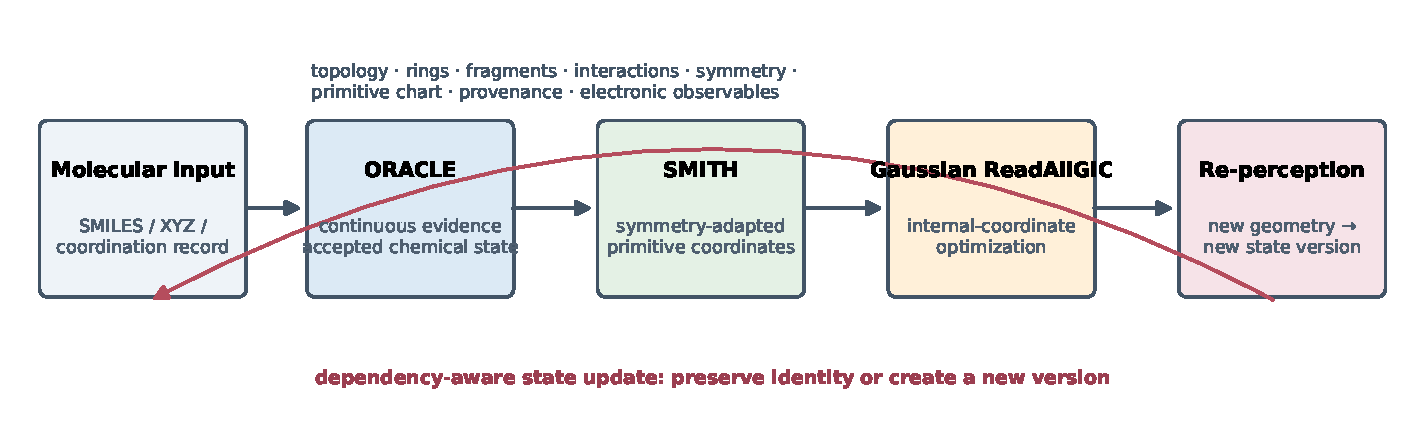
\includegraphics[width=0.98\linewidth]{figures/oracle_workflow_state_transfer.pdf}
\caption{State transfer from perception through coordinate construction and re-perception.}
\label{fig:workflow-state-transfer}
\end{figure*}

\rev{Two chemically demanding demonstrations anchor the validation.  The
transition-state examples test whether one perception protocol can span
ring opening, dissociation, insertion, torsional isomerization and
rearrangement.  Fe$_4$S$_4$Cl$_4$ tests whether the same state can encode a
polynuclear coordination topology whose 22 accepted edges are not recoverable
from simple organic-valence rules.  Figures~\ref{fig:baker-ts-examples} and
\ref{fig:fe4s4cl4-topology} place these two cases at the center of the
subsequent quantitative audits.}

\begin{table}[t]
\centering
\scriptsize
\caption{Four discriminating tests of the persistent chemical state.}
\label{tab:evidence-summary}
\begin{tabularx}{\linewidth}{@{}lX@{}}
\toprule
Test & What it establishes \\
\midrule
Transition-state geometries (25 cases) & One local perception/chart protocol spans ring opening, dissociation, insertion, torsional isomerization and rearrangement. \\
Fe$_4$S$_4$Cl$_4$ ($C_{3v}$) & Explicit coordination state preserves a non-obvious 22-edge polynuclear topology and the rank of the nonredundant internal coordinates. \\
Seven-target leave-one-out transfer & SWITCH, ORACLE and the primitive chart transport reference information to held-out structures; thiazole gives the representative quantitative case. \\
State-blind electronic control & At fixed nuclear geometry, graph-only output is unchanged across state and environment changes, whereas ORACLE updates CM5, Mayer and spin observables. \\
\bottomrule
\end{tabularx}
\end{table}

\begin{table}[t]
\centering
\scriptsize
\caption{Evidence hierarchy used in the validation.}
\label{tab:evidence-hierarchy}
\begin{tabularx}{\linewidth}{@{}lXX@{}}
\toprule
Evidence class & Comparison & Interpretation \\
\midrule
Efficiency check & Persistence versus forced re-perception & Same chemical result with modestly faster state reuse. \\
Capability & Transition-state geometries and Fe$_4$S$_4$Cl$_4$ & Tasks and topologies represented natively in the ORACLE state. \\
Differentiation & State-blind fixed-geometry control & Same graph, state-dependent CM5/Mayer/spin output. \\
\bottomrule
\end{tabularx}
\end{table}

\subsection{One state survives geometric and representational stress}

Figure~\ref{fig:validation} summarizes the elementary validation through
eleven predeclared topology cases spanning isolated, fused, spiro, cage and
metallocene graphs.  In every case ORACLE recovers the expected bond count,
cycle-space rank, elementary cycle sizes, aromatic-atom count and
connected-fragment count.  The aromaticity
rule combines planarity, local $p$-orbital eligibility and $4n+2$ counting,
with separate criteria for fused conjugated components and
metal-coordinated $\eta^5$ rings.  Aromatic assignment requires the complete
set of chemical criteria.

Seven molecular benchmarks from $C_{2v}$ to $I_h$ recover complete operation
sets and atom permutations, including $D_{5h}$, $D_{5d}$, $T_d$, $O_h$ and the
120 operations of $I_h$.  A separate generic audit spans 45 finite groups:
all six axial families for $n=2$--6, $S_4$ through $S_{12}$, the three
low-order groups, and all seven tetrahedral, octahedral and icosahedral
families.  For every case ORACLE verifies identity, exact order, inverse and
matrix--permutation closure after a fixed three-dimensional rotation and
translation; the coordinate layer then constructs the complete finite character sequence
from that same action.  The intermediate $D_5$ ferrocene geometry is an
additional discriminating regression: it recovers all ten operations, and the
resulting 57 internal coordinates close the full vibrational rank.

For distorted formaldehyde, a threshold sweep distinguishes the onset of a
stable quasi-$C_{2v}$ plateau from the smaller-$\tau$ $C_s$ result.  The
selected $\tau=5\times10^{-4}$~\AA\ is the smallest plateau value with adequate
residual margin; projection requires only
$8.07\times10^{-5}$~\AA\ maximum displacement and reanalysis returns exact
$C_{2v}$ to numerical precision.

The continuous descriptors are invariant to rigid motion and atom order at numerical precision
for water, benzene and methane.  A sampled $2\times10^{-4}$~\AA\ local
displacement produces a correspondingly small descriptor response while the
discrete topology remains unchanged, completing the local regression
contract around the sampled geometries.

\begin{figure*}[htbp]
\centering
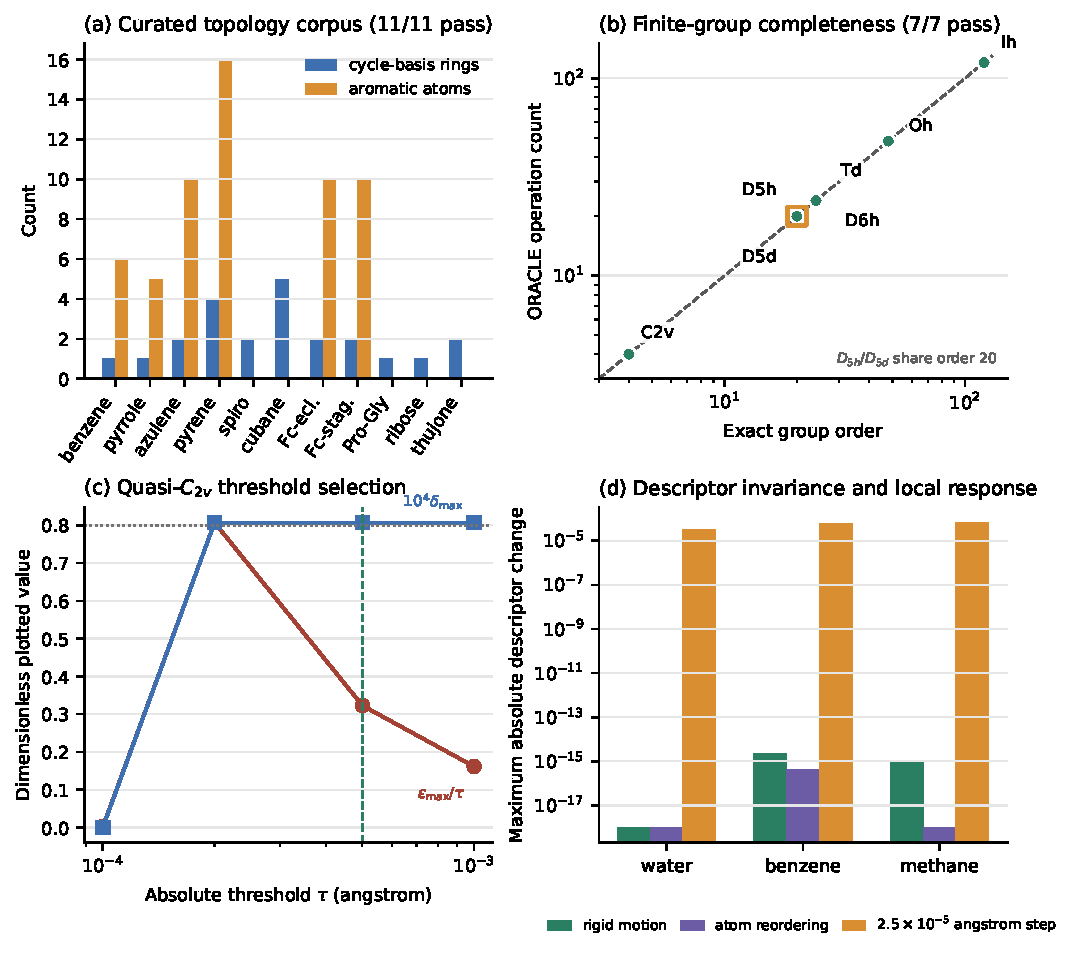
\includegraphics[width=\linewidth]{figures/oracle_validation_summary.pdf}
\caption{Validation summary. Panels (a)--(d) show topology and aromaticity, finite-group action, quasi-symmetry threshold selection, and descriptor invariance with local response.}
\label{fig:validation}
\end{figure*}

An additional ethanol check connects low- and high-information states.
Complete-link clustering of the seven descriptor components yields five
transparent classes---the two carbon environments, oxygen, carbon-bound
hydrogen and hydroxyl hydrogen---and those classes remain unchanged from one
quarter to twice the declared thresholds as well as after atom-order
reversal.  The result illustrates an availability-level contract that remains
auditable across different information levels.

\subsection{The state is executable at practical scale}

The compiled path keeps the additional chemical evidence affordable.  Pair
geometry, continuous refinement,
accepted-graph construction, cyclic-core restriction and independent-cycle
selection are evaluated together, while lazy materialization avoids dense
matrices when a consumer requires topology alone.  Relative to the equivalent
Python reference, this path is 5.74-fold faster at the median over six
systems, ranging from 2.24-fold for water to 9.93-fold for paclitaxel; on the
reported arm64 host, the vancomycin time decreases from 36.5 to 4.0~ms.
The compiled and Python paths return identical edges and canonical cycles,
the wider audit retains cyclic-core/
Horton equivalence for 4991/4991 molecules, and all graph, ring-rank and
benchmark checks pass for 346/346 structures.  Exact environments, raw
timings, compiled-build metadata and the Python fallback are documented in
the Supporting Information.

An independent RDKit comparison places the graph and cycle machinery on the
scale of current cheminformatics practice.
\cite{rdkit_book_2026}  Agreement counts and disagreement records are reported
in the Supporting Information.  The comparison establishes graph and cycle
conformance for equilibrium structures.  The transition-state examples extend
this representation by retaining forming and breaking contacts as typed
evidence and by selecting among primitive charts through the Wilson-$B$
condition number before downstream coordinate construction.

\subsection{Quantum mechanics feeds the chemical state back}

Three complementary chemical domains make the perception--QM connection
concrete.  Aromatic systems test how total Mayer orders refine conjugation,
open-shell systems add the spatial distribution of spin, and transition-metal
complexes test the same population contract across all-electron and
effective-core-potential descriptions.

Chemical discrimination is examined separately on a stratified corpus of 58
frozen structures spanning benzenoid, heteroaromatic, fused, nonbenzenoid and
boundary systems together with nonaromatic controls.  Every geometry passes
the declared numerical gate.  The present method and geometry-first RDKit
return identical aromatic-atom sets in 58/58 cases; the same agreement is
obtained when RDKit receives the accepted covalent graph.  The exact-match
fraction is therefore 1.00, with a two-sided Wilson 95\% interval of
0.94--1.00, and the mean and minimum Jaccard indices are both 1.00.
Cyclopropenone and acenaphthylene are included explicitly as discriminating
boundary cases.  The result measures conformance between independent
implementations over the declared corpus.  The full atom sets, strata, source
hashes and environment are reported in the Supporting Information.

The electronic-feedback route is tested independently on 18 neutral doublets
distributed over nine electronic classes: localized, unsaturated and
conjugated cyclic carbon radicals, heteroatom-substituted carbon radicals,
aryloxy, carbonyl, nitroxide, nitrogen-centered and peroxy
systems.  All unrestricted Kohn--Sham PBE0 (UKS-PBE0)/def2-TZVP L0 calculations converge; the Hirshfeld
$\alpha-\beta$ populations satisfy the unit-spin sum exactly after the
declared $2\times10^{-4}$ quadrature gate, and
$\langle S^2\rangle$ ranges from 0.754 to 0.805.  The absolute-spin
participation spans 1.38--4.85 atoms, with a bootstrap 95\% interval of
2.00--2.96 atoms for its corpus mean.  Maximum absolute
$\alpha-\beta$ Mayer components span 0.002--0.46, with a corresponding
bootstrap mean interval of 0.068--0.23.  In phenyl, the
six ring bonds have total Mayer orders of 1.408--1.514 while their
spin-selective components remain at or below 0.047; the L0 state therefore
separates aromatic bond equalization from the localized open-shell response.
Together, the nine-class stratification and bootstrap intervals provide a
quantitative characterization of the declared open-shell set, with paired
observations resolving the electronic response within each class.  They
establish the reverse, quantum-mechanical leg of the
perception--QM connection: electronic observables update the chemical state
before geometry refinement and the production calculation.
Functional conformance is additionally checked on macOS/arm64 and
Linux/x86-64, with environment-specific records; timings are compared only
within the same host.

State-specific electronic observables provide a direct test of the
bidirectional contract.  On the same ORACLE-perceived geometry, CH$_2$ was
evaluated as both a singlet and a triplet, and O$_2$ as a triplet.  The CH$_2$
C--H Mayer order changes from 0.938 to 0.951 and the carbon CM5 charge from
$-0.179$ to $-0.201~e$ on changing the multiplicity.  A complementary
time-dependent density-functional theory in the Tamm--Dancoff approximation with PBE0 (TDA/PBE0) gives a singlet S$_1$ excitation at
3.98 eV; the carbon and oxygen CM5 charges change from $+0.053$ and
$-0.290~e$ in the ground state to $-0.307$ and $+0.003~e$, while the C=O
Mayer order decreases from 2.098 to 1.445.  These state-dependent changes
illustrate why CM5/Mayer observables can influence subsequent atom typing,
charge assignment and force-field parameter selection.  For uracil, the two
carbonyl Mayer orders change from 2.072 and 2.037 in S$_0$ to 1.966 and 1.828
in S$_1$; the S$_0$ values become 2.049 and 1.977 in aqueous conductor-like
polarizable continuum model (C-PCM).  The
C4=O4 carbonyl is more strongly perturbed in both comparisons, demonstrating
state- and environment-dependent parameter selection.  The
complete records are provided in the Supporting Information.

The fixed-geometry comparisons define a direct boundary with graph-only
cheminformatics. Changing multiplicity, electronic state or dielectric
environment does not change the nuclear graph, so a conventional graph
perception layer would return the same structural object. ORACLE retains the
electronic and environmental context and propagates the resulting CM5, Mayer
and spin observables into the chemical state. This is the mechanism by which
non-obvious open-shell states, excited states and solvent-aware parameter
selection remain distinguishable downstream.

A three-level sensitivity calculation quantifies the range of the L0 closure.
At the same ORACLE geometries, PBE0/def2-SVP, PBE0/def2-TZVP, and
B3LYP/def2-TZVP give formaldehyde S$_1$ C=O Mayer orders of 1.459, 1.445,
and 1.430, respectively, while the corresponding S$_0$ values are 2.106,
2.098, and 2.092. For uracil, the two S$_1$ carbonyl orders are 1.966/1.828
at PBE0/def2-TZVP, compared with 2.072/2.037 in S$_0$; the functional/basis
range is reported in the Supporting Information. The state effect is
therefore larger than the level variation in these examples, while the level
variation remains large enough to justify preserving the declared functional,
basis, and solvent metadata with the chemical state.

The state-blind control holds the nuclear geometry and covalent graph fixed and
assigns no state-dependent electronic observables. Its structural output is
therefore unchanged, whereas ORACLE records a carbon CM5 change of $-0.022~e$
and a mean C--H Mayer change of $+0.013$ for CH$_2$ singlet to triplet. For
formaldehyde S$_0$ to S$_1$, the corresponding carbon and oxygen CM5 changes
are $-0.360$ and $+0.293~e$, and the C=O Mayer change is $-0.652$. The control
isolates the scientific consequence of retaining electronic state at fixed
geometry and shows how the persistent state records changes that a
geometry-only route leaves unrepresented.  The numerical consequences are
collected in Figure~\ref{fig:state-comparison} and
Table~\ref{tab:state-level-sensitivity}.
This is not a performance comparison between competing implementations of the
same electronic task: standard graph-only toolkits do not compute Mayer spin
components or state-specific electronic observables.  The comparison therefore
tests whether the chemical state retains information that a graph-only object
cannot contain.

At fixed nuclear geometry, any perception layer limited to the covalent graph---including
RDKit, Open Babel, or the Chemistry Development Kit (CDK) in their standard operation---returns an unchanged
structural object for all four comparisons in Table~\ref{tab:state-chemical-consequences}.
ORACLE differentiates them because electronic-state and dielectric metadata are
part of the persistent object; the resulting CM5, Mayer, and spin changes are
therefore state evidence rather than a geometry-only modeling choice.

\begin{table}[htbp]
\centering
\scriptsize
\caption{State-dependent chemical evidence at fixed nuclear geometry.}
\label{tab:state-chemical-consequences}
\begin{tabularx}{\linewidth}{@{}p{0.16\linewidth}p{0.17\linewidth}p{0.18\linewidth}p{0.19\linewidth}X@{}}
\toprule
\textbf{Case} & \textbf{CM5 change} & \textbf{Mayer change} &
\textbf{State object} & \textbf{Downstream use}\\
\midrule
CH$_2$ S$_0\!\to$ T$_1$ & $\Delta q_C=-0.022~e$ & $\Delta\mathrm{BO}_{\mathrm{C-H}}=+0.013$ & synthon/$Z_i^{\mathrm{eff}}$ update & spin-aware atom typing and parameter routing\\
H$_2$CO S$_0\!\to$ S$_1$ & $\Delta q_C=-0.360~e$ & $\Delta\mathrm{BO}_{\mathrm{C=O}}=-0.653$ & carbonyl synthon update & excited-state bond and force-field selection\\
Uracil S$_0\!\to$ S$_1$ & state-specific vector & $\Delta\mathrm{BO}_{\mathrm{C4=O4}}=-0.209$ & carbonyl synthon/$Z_i^{\mathrm{eff}}$ update & inequivalent carbonyl parameter selection\\
Uracil gas $\to$ C-PCM & solvent-specific vector & $\Delta\mathrm{BO}_{\mathrm{C4=O4}}=-0.060$ & environment-aware synthon & solvent-aware equilibrium parameters\\
\bottomrule
\end{tabularx}
\end{table}

\begin{table}[htbp]
\centering
\scriptsize
\caption{State and electronic-level sensitivity at fixed nuclear geometries.}
\label{tab:state-level-sensitivity}
\begin{tabular}{@{}lccc@{}}
\toprule
Case & PBE0/def2-SVP & PBE0/def2-TZVP & B3LYP/def2-TZVP \\
\midrule
CH$_2$ S$_0$: C--H Mayer & 0.944 & 0.938 & 0.936 \\
CH$_2$ T$_1$: C--H Mayer & 0.969 & 0.951 & 0.951 \\
H$_2$CO S$_0$: C=O Mayer & 2.106 & 2.098 & 2.092 \\
H$_2$CO S$_1$: C=O Mayer & 1.459 & 1.445 & 1.430 \\
Uracil S$_0$: two C=O Mayer & 2.135/2.067 & 2.072/2.037 & 2.081/2.040 \\
Uracil S$_1$: two C=O Mayer & 2.042/1.881 & 1.966/1.828 & 1.976/1.825 \\
\bottomrule
\end{tabular}
\end{table}

\begin{figure}[htbp]
\centering
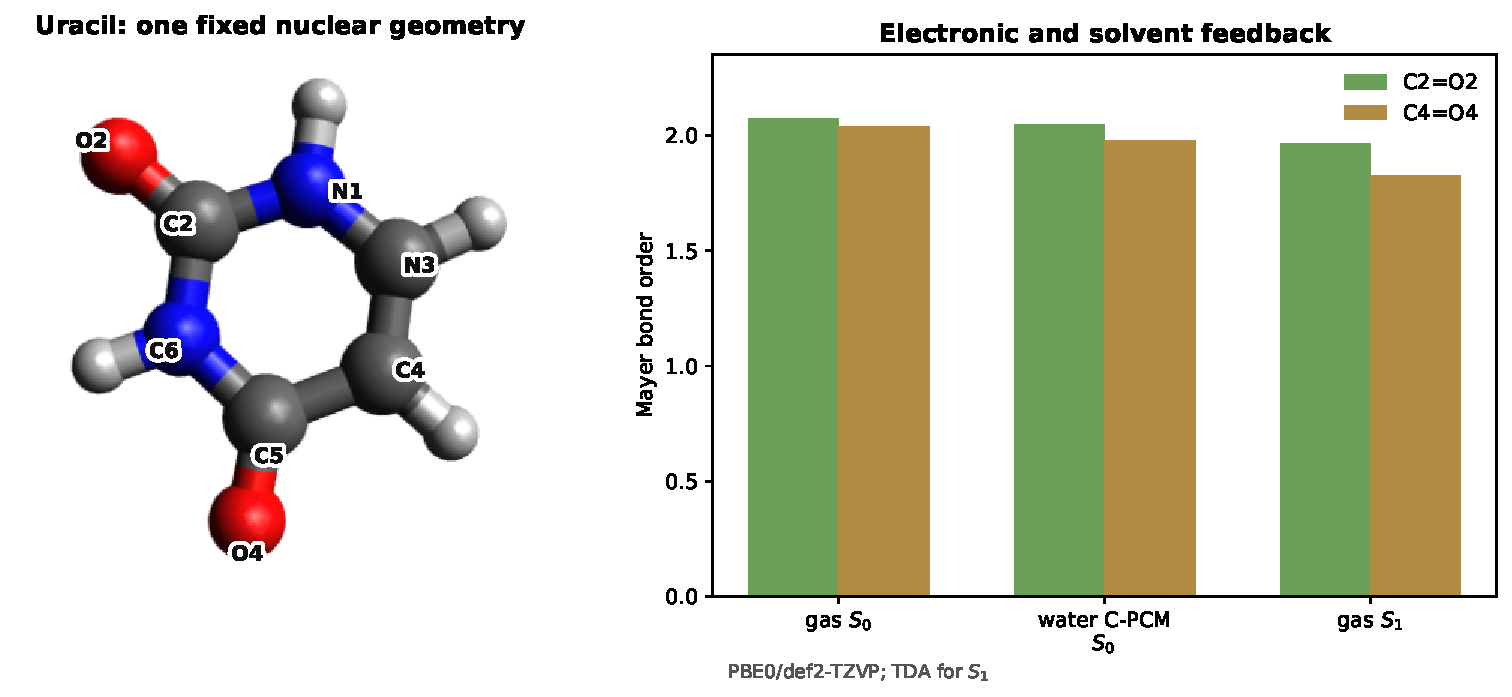
\includegraphics[width=\linewidth]{figures/oracle_state_comparison.pdf}
\caption{Uracil at fixed geometry; the C4=O4 bond is most strongly perturbed.}
\label{fig:state-comparison}
\end{figure}

The fixed-geometry electronic comparison is illustrated in Figure~\ref{fig:state-comparison}
and quantified in Table~\ref{tab:state-level-sensitivity}.

The transition-metal examples complete this electronic picture
(Figure~\ref{fig:l0-metal-complexes}).  All-electron $D_{5h}$ ferrocene gives
$q_{\mathrm{Fe}}=+0.984~e$ and ten equivalent Fe--C Mayer orders of 0.441.
With the native def2 effective core potential, $C_{2v}$ cisplatin gives
$q_{\mathrm{Pt}}=+0.657~e$, Pt--Cl 0.802 and Pt--N 0.520.  Both
fixed-geometry calculations converge and conserve charge within
$3\times10^{-16}~e$, showing that the same perceived state and population
analysis remain coherent across distinct coordination and relativistic
regimes.

\rev{A more demanding coordination example is the neutral singlet
Fe$_4$S$_4$Cl$_4$ cluster in $C_{3v}$ symmetry (12 atoms).  Its topology is
not recoverable from a simple ligand-counting rule: the accepted graph
contains the six Fe--Fe edges of the Fe$_4$ tetrahedron, twelve Fe--S edges
forming the cubane-like core, and four terminal Fe--Cl edges, for 22 accepted
edges in total, with no S--S or Cl--Cl edges.  The enriched XYZ record stores
this graph, the continuous bond-order components, and the requested $C_{3v}$
symmetrization before coordinate construction.  The independent coordinate output
starts from 182 primitive candidates, filters these to 136 admissible
candidates, and retains 30 frozen internal coordinates that reach the complete non-linear rank
$3N-6=30$; matrix--permutation closure is confirmed, with 21 totally
symmetric $A_1$ coordinates.
This case exercises the enriched coordination representation and shows why
explicit connectivity, symmetry, and primitive-coordinate provenance are
needed when a polynuclear topology is chemically non-obvious.}

\begin{figure*}[htbp]
\centering
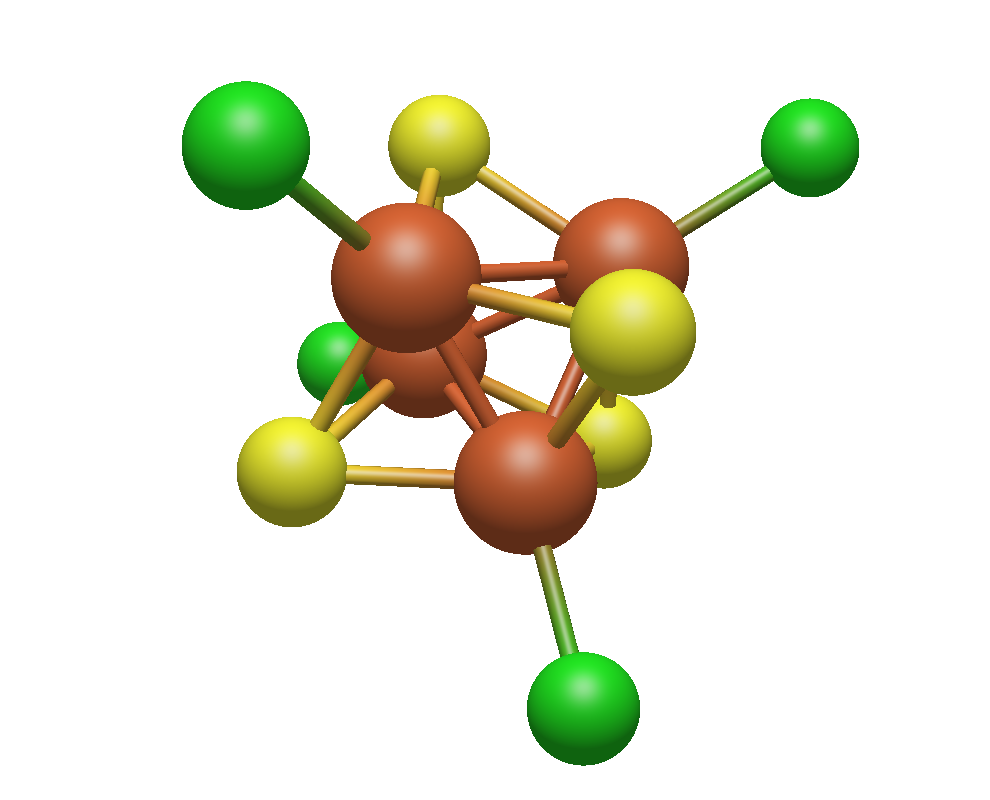
\includegraphics[width=0.62\linewidth]{figures/Fe4S4Cl4_C3v_Avogadro.png}
\caption{Neutral singlet Fe$_4$S$_4$Cl$_4$ coordination topology in $C_{3v}$ symmetry.}
\label{fig:fe4s4cl4-topology}
\end{figure*}

\begin{figure*}[htbp]
\centering
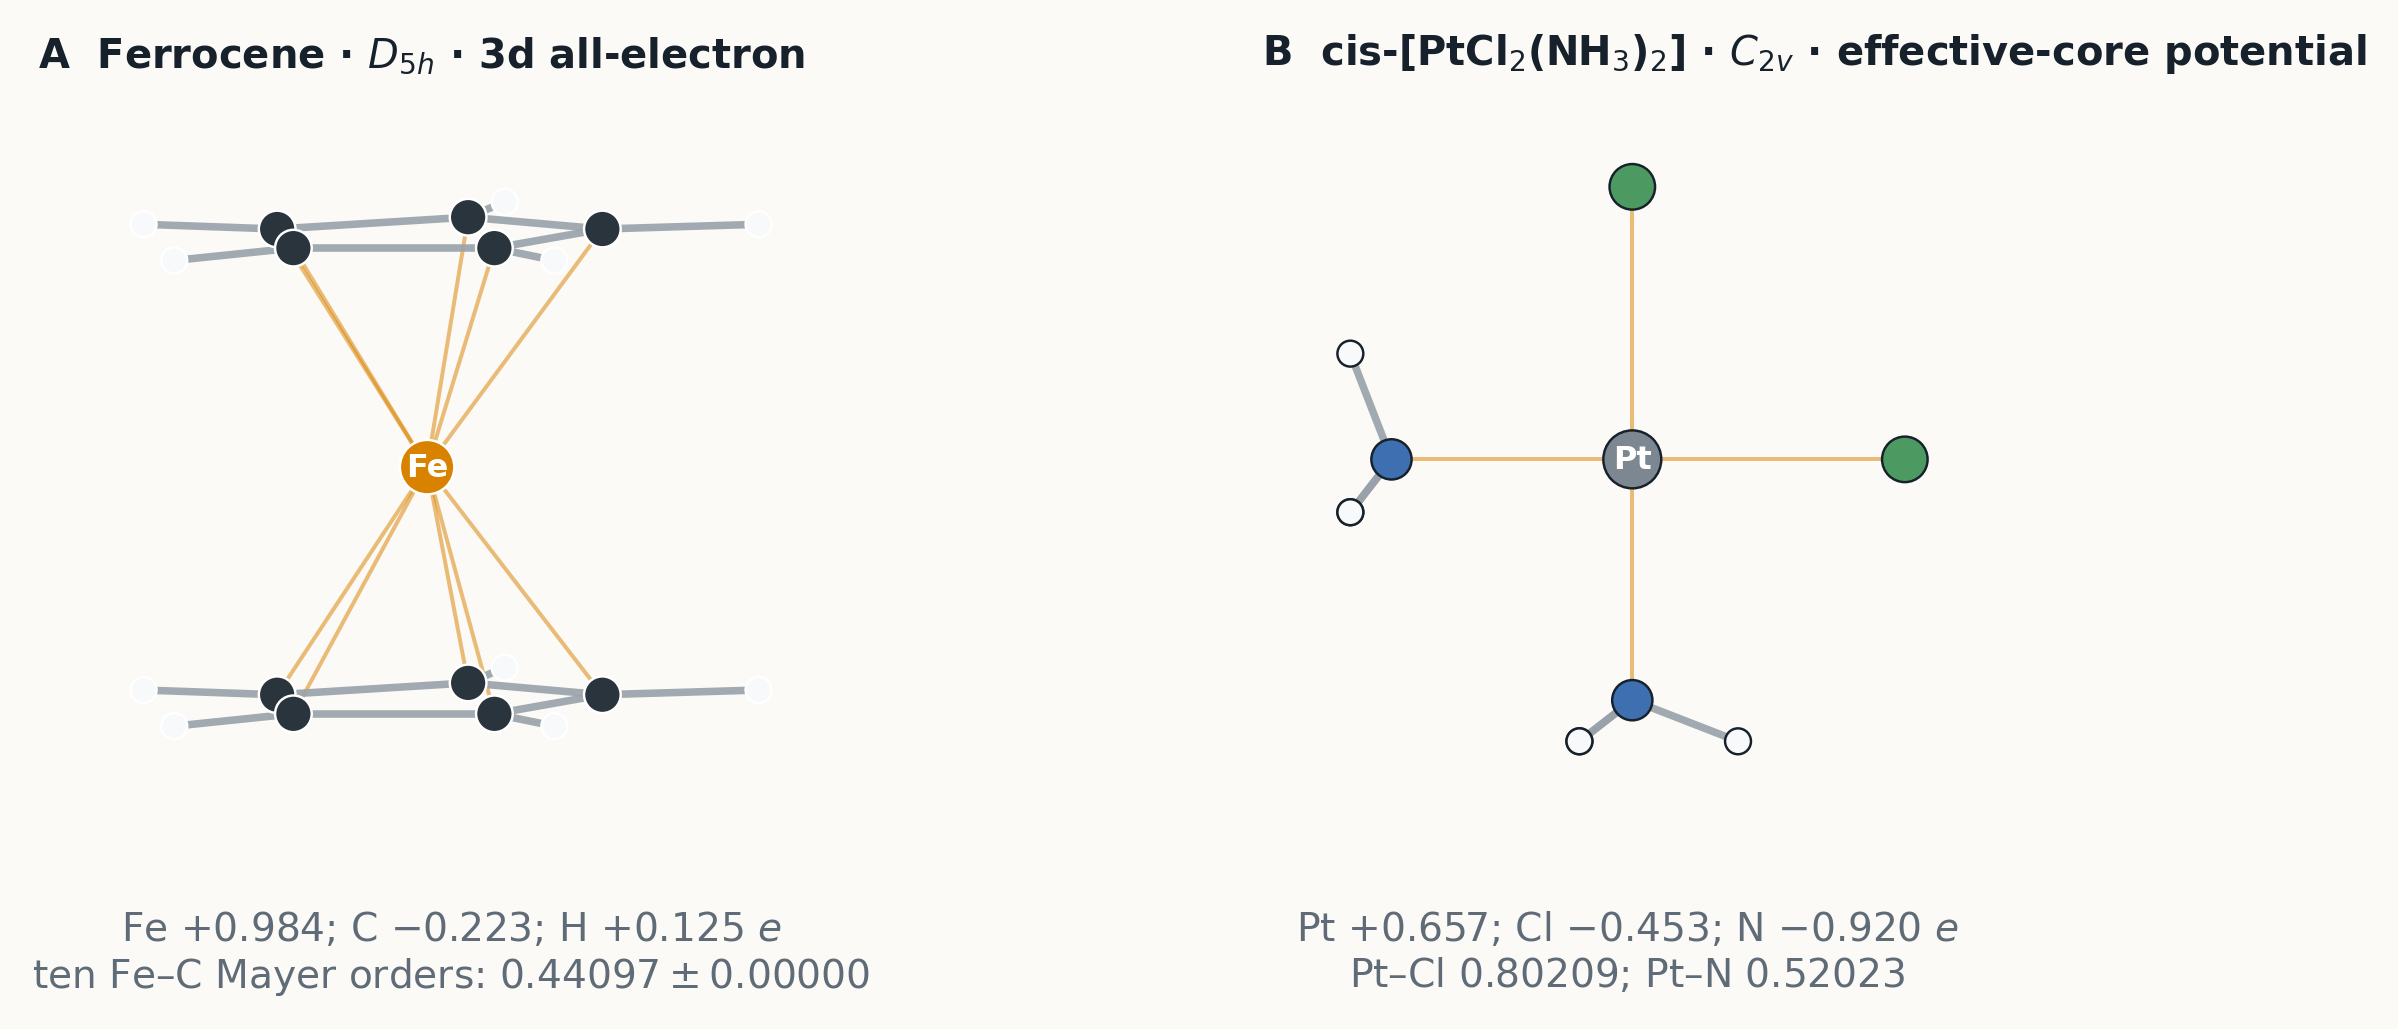
\includegraphics[width=\linewidth]{figures/oracle_l0_metal_complexes.png}
\caption{Baseline populations at fixed geometry. Panels (A)--(B) show ferrocene and cisplatin, respectively.}
\label{fig:l0-metal-complexes}
\end{figure*}

\subsection{Chemical consequences of continuous perception}

The atomic synthon is the local chemical object that carries continuous
evidence into subsequent operations.  Its effective atomic number provides a
compact coordinate for comparing environments while preserving elemental
identity.  This combination makes related atoms clusterable without erasing
gradual changes in geometry or electronic population, and supports atom
typing, fragment construction and parameter retrieval.  The same descriptors
remain meaningful when the nuclear geometry is unchanged but the electronic
state or environment changes, as shown for CH$_2$, formaldehyde, uracil and
gas/solvent comparisons.  Reactive contacts become typed evidence for
transition-state charts, while continuous coordination retains non-obvious
metal environments such as Fe$_4$S$_4$Cl$_4$.
The relationship between elemental identity, local environment and
$Z_i^{\mathrm{eff}}$ is summarized in Figure~\ref{fig:effective-atomic-number}.

\begin{figure*}[htbp]
\centering
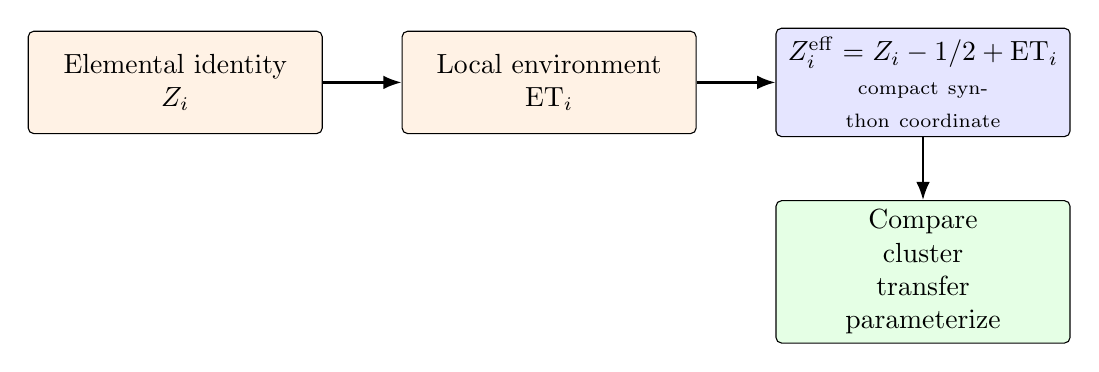
\begin{tikzpicture}[>=Latex, node distance=8mm and 10mm,
  zbox/.style={draw, rounded corners=2pt, align=center, minimum height=13mm,
    text width=35mm, fill=orange!10}, arr/.style={->, thick}]
\node[zbox] (element) {Elemental identity\\$Z_i$};
\node[zbox, right=of element] (env) {Local environment\\$\mathrm{ET}_i$};
\node[zbox, right=of env, fill=blue!10] (zeff) {$Z_i^{\mathrm{eff}}=Z_i-1/2+\mathrm{ET}_i$\\\scriptsize compact synthon coordinate};
\node[zbox, below=of zeff, fill=green!10] (uses) {Compare\\cluster\\transfer\\parameterize};
\draw[arr] (element) -- (env); \draw[arr] (env) -- (zeff); \draw[arr] (zeff) -- (uses);
\end{tikzpicture}
\caption{Role of the effective atomic number in the ORACLE chemical module.}
\label{fig:effective-atomic-number}
\end{figure*}

\subsection{Test case I: traceable [6]helicene assembly from overlapping tiles}

Fragment-based construction uses shared geometry to determine relative
placement.  This information is essential for fused, polycyclic and
stereochemically congested targets.  ORACLE therefore treats overlap as the
geometrical contract.  Every fragment
after the seed must share at least three non-collinear heavy atoms with the
assembled structure and add at least one new atom.  The shared coordinates
define a proper Kabsch rigid fit; collinear overlaps are rejected, and the
source path, atom mapping, new/overlap sets and fit root-mean-square deviation
(root-mean-square deviation, RMSD) are serialized.  A
deterministic beam search selects the covering set and a joint rigid-pose fit
then optimizes all selected placements simultaneously.

[6]Helicene is a discriminating test with simple connectivity and a
nonplanar three-dimensional structure.  A planar
polycyclic drawing contains a severe terminal steric conflict, whereas the
physical structure is helical and chiral.  The local cache of the published
2025 chemical building-block library (LCB25) contains a naphthalene geometry from its
companion input level,\cite{LCB25_2025} with 18 atoms including hydrogens, below the
literal 20-atom limit.  The internal SWITCH parser described in
Section~\ref{sec:computational-details} identifies five naphthalene occurrences in the
target [6]helicene graph.  The first covers 10 carbon atoms; each subsequent
occurrence shares a complete six-carbon ring and adds four carbons.  The five
placements therefore cover all 26 target heavy atoms, while every step is
more strongly determined than a single-bond link (Figure~\ref{fig:overlap-assembly}).

\begin{figure*}[htbp]
\centering
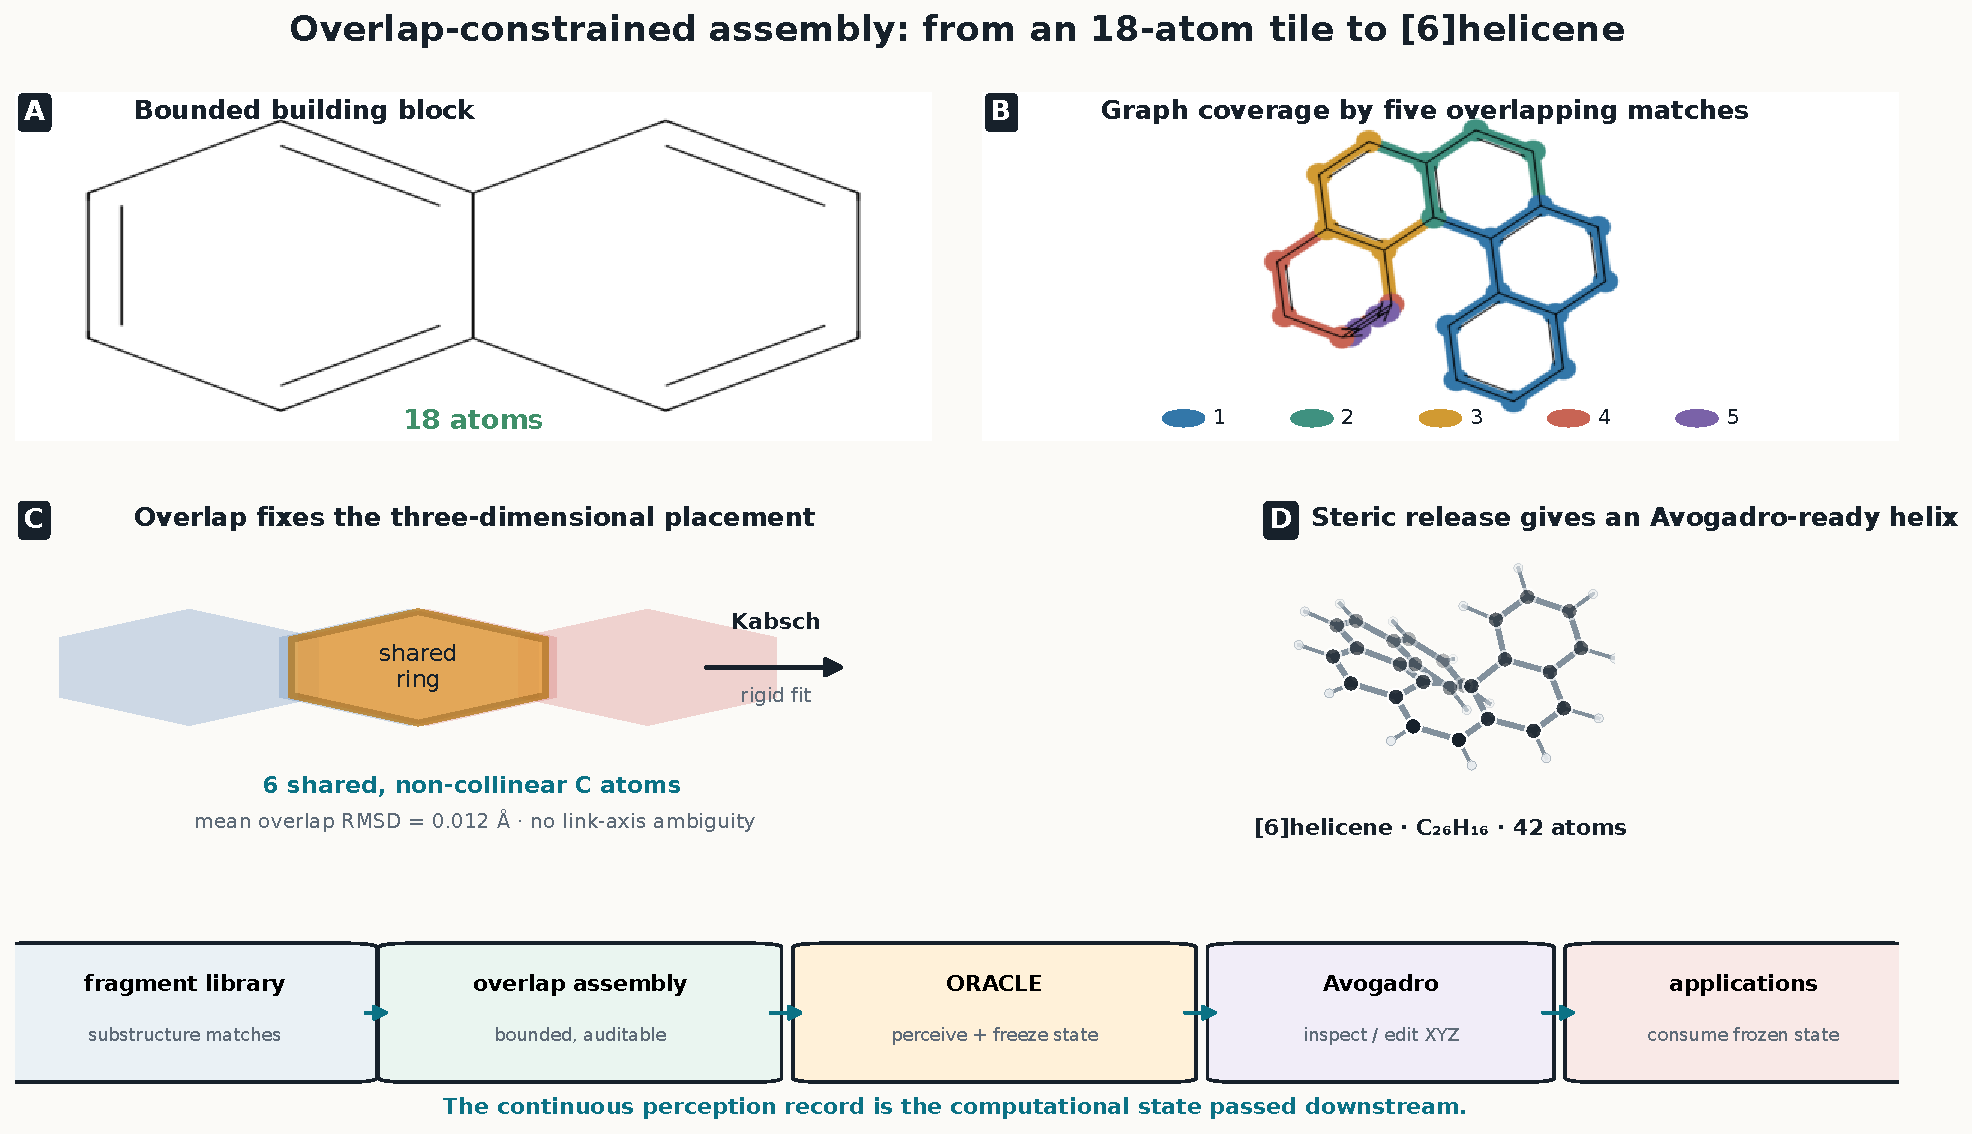
\includegraphics[width=\linewidth]{figures/oracle_overlap_assembly.pdf}
\caption{Overlap-constrained [6]helicene construction. Panels (A)--(D) show the building block, graph coverage, three-dimensional placement, and steric release.}
\label{fig:overlap-assembly}
\end{figure*}

The four non-seed alignments have RMSDs 0.014, 0.013, 0.013 and
0.011~\AA; the joint pose fit converges in 18 iterations and passes the
strict 0.35~\AA\ quality gate cleanly.  A small deterministic
displacement normal to the initially assembled aromatic scaffold breaks the
exactly planar steric saddle; Geometry, Frequency, Noncovalent force field (GFN-FF) relaxation releases the terminal
contact while preserving the fragment-derived geometry.  Hydrogens are
added only after complete heavy-atom coverage.  The resulting
C$_{26}$H$_{16}$ structure contains 42 atoms, and an ORACLE reimport recovers
47 covalent bonds, six rings and $C_2$ symmetry.  The default output is strict
XYZ for direct ORACLE and Avogadro use; the adjacent
\texttt{oracle.xyz.assembly.v1} JavaScript Object Notation manifest stores
mappings, provenance,
beam-search and pose diagnostics, and the quality decision.
The assembled structure is shown in Figure~\ref{fig:overlap-assembly}.

\paragraph{A reusable carbohydrate subset.}
The same construction also applies beyond fused aromatics.  The 2026 chemical
building-block library (LCB26) adds high-level equilibrium
structures of representative sugars and their oxygenated fragments.
The present carbohydrate-focused set contains xylose, erythrose, erythrulose,
threose and fructose together with glycidaldehyde, glycidol, glycolaldehyde,
glyceraldehyde, glycerol and 1,3-dihydroxyacetone.  These entries form a
connected family of ring, polyol, carbonyl and hydroxymethyl environments.
ORACLE assembles $\alpha$-D-glucopyranose from D-xylose
\texttt{aconf10} and glycerol \texttt{C5}: the placements share four heavy
atoms, cover all 12 target heavy atoms and give a maximum overlap RMSD of
0.33~\AA.  On the rounded values shown, this corresponds to approximately
24--30 times the 0.011--0.014~\AA\ range for
helicene and approaches the declared 0.35~\AA\ boundary.  Thus helicene probes
near-rigid overlap, whereas glucose probes flexible placement; both recover
the intended ring and a valid persistent state.  Library composition and
complete records are given in the Supporting Information.

A leave-one-chemical-identity-out experiment tests reconstruction from an
independent donor by withholding
1,3-dihydroxyacetone \texttt{c,c} and excludes any donor with the same
constitution.  The target SMILES and conformer label are fixed before
construction, and the hidden high-level geometry is reserved for scoring.  ORACLE
selects an erythrulose subgraph and reconstructs the specified cis/cis
hydroxyl arrangement with heavy- and all-atom RMSDs of 0.067 and
0.144~\AA, respectively; the bond-length root-mean-square (RMS) error is
14.0~m\AA.  A deterministic 20-start Experimental-Torsion Knowledge Distance
Geometry, version 3, calculation followed by the Merck force field provides a
fragment-free baseline and
gives 0.077 and 0.157~\AA\ and 13.1~m\AA.  The comparable skeleton and bond
errors isolate the added chemical information supplied by the fragment
route: in this case it primarily improves hydroxyl orientation.  The
reconstructed hydroxyl torsions remain cis at $+16.3^\circ$ and
$+17.7^\circ$, while the reference values are $0^\circ$; ORACLE accordingly
assigns $C_1$, while the reference is $C_{2v}$.  This predeclared, held-out
conformer provides a quantitative test of reconstruction and stereochemical
auditing through the residual torsional distortion and associated symmetry
change.

\paragraph{Frozen peptide population synthesis.}
Gly--Ala--Gly extends the same idea to electronic populations while keeping
the geometry frozen.  The reference is a completely extended, zero-contact
configuration, so $s_c(\mathbf R_{\mathrm{ref}})=0$ and the assembled CM5
populations directly define $\mathbf q^0$.  Any subsequently accepted
hydrogen bond adds donor polarization, acceptor polarization and charge
transfer through its continuous dimer rule.  The same parser generates the
stereochemical Cartesian structure; ORACLE assigns residue cores, expands
each by two covalent shells and caps the outer halo.  Charges and Mayer orders
are taken from the deepest owned interiors, while repeated halo observations
measure boundary sensitivity.

Three L0 fragment calculations and an independent calculation of the complete
frozen molecule provide a direct audit (Figure~\ref{fig:gly-ala-gly}).  The
assembled CM5 charges differ from the direct result by 0.003~$e$
root-mean-square and 0.010~$e$ at most, while restoring exact molecular
neutrality requires a maximum correction of
$3.90\times10^{-4}$~$e$.  The core-owned construction avoids averaging boundary
and interior populations alike.
and interior populations alike.  Assigning ownership to the core removes cap
contamination and preserves both geometry and electronic level.

Neutral fast-multipole source groups are constructed only after the molecular
CM5 and Mayer state has been assembled and its total charge restored by the
minimum-displacement projection.  The QM fragments themselves are therefore
overlapping electronic environments; the neutral electrostatic groups
represent the assembled molecular state.
Separating these two partitions preserves local chemistry during electronic
reconstruction and subsequently suppresses the monopole term of neutral
groups during far-field evaluation.

\begin{figure*}[htbp]
\centering
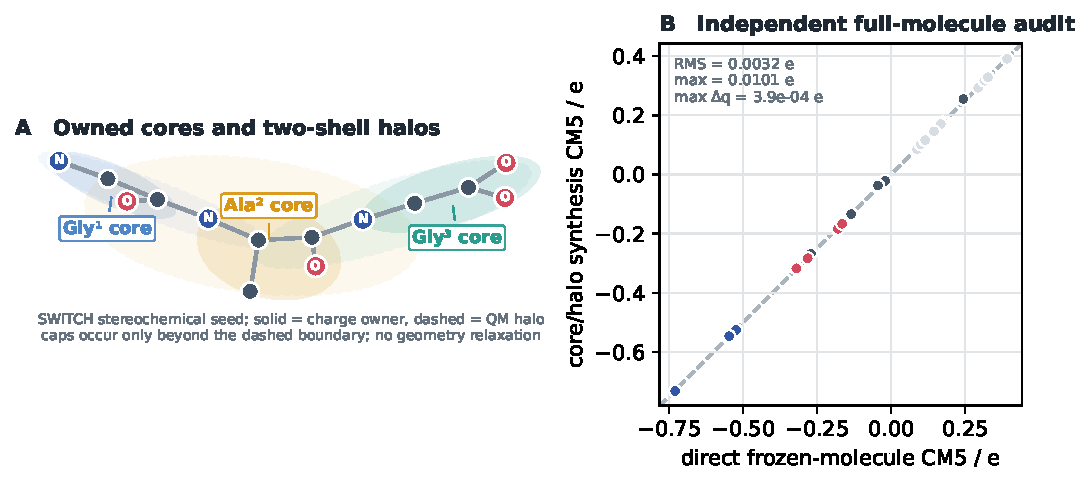
\includegraphics[width=\linewidth]{figures/oracle_gly_ala_gly_fragments.pdf}
\caption{Frozen Gly--Ala--Gly population synthesis from overlapping fragments. Panels (A)--(B) show owned cores with halos and the full-molecule audit.}
\label{fig:gly-ala-gly}
\end{figure*}

Here the service layer supplies stereochemical parsing, matching, valence
completion and deterministic hydrogen placement, while GFN-FF provides the universal initial
relaxation, chosen for periodic-table coverage and improved accuracy over the
Universal Force Field.\cite{gfnff_2020,uff_1992}  ORACLE then freezes topology, symmetry, local descriptors,
atom types and primitive coordinates, keeping the chemical state independent
of parser, seed generator and force field.

The current 2025 library cache contains 776 local Cartesian files across its
three reference-level collections\cite{LCB25_2025} and already
supplies aromatic tiles such as benzene,
naphthalene, acenaphthylene and acenaphthene.  The helicene construction
identifies useful additions more precisely than a request for ``larger
fragments'': compact aza-aromatic, hetero-fused, saturated-ring, carbonyl-ring
and cis/trans junction tiles with non-collinear overlaps.  Each record should
retain charge/multiplicity provenance and its high-level geometry source.

All uses of this library in the present work---saccharin retrieval,
leave-one-out validation,
benchmarks and overlap assembly---resolve records through the same
manifest-managed local cache.  The cache is populated once from the published
archives and records their hashes.  The reference subset is one deterministic
set of 331 usable coupled-cluster singles and doubles with perturbative
triples [CCSD(T)] geometries extrapolated to the complete-basis-set (CBS)
limit and including core--valence (CV) contributions, denoted
CCSD(T)/CBS+CV throughout the
work.\cite{LCB25_2025}  This state-of-the-art structural level is the source
of the library's accuracy; ORACLE separately audits whether its chemical
coverage supports a query.  The scope of the library differs from that of the
formulation.
Continuous perception, coordination, local descriptors, and the L0 electronic interface
are defined across the periodic table, whereas the published LCB25 accurate
structure library is deliberately restricted to the elements essential for
the chemistry of life: H, C, N, O, F, P, S, and Cl.  Accordingly, every
LCB25 retrieval, transfer, and reconstruction test reported here uses these
elements.  ORACLE perception and the fixed-geometry L0 examples retain their
periodic-table scope.

\subsection{Test case II: topology at molecular scale}

Four demanding structures test perception directly from element labels and
archived Cartesian coordinates.  ORACLE constructs their bonds, rings and
atom selections internally (Figure~\ref{fig:large-systems}).

\begin{figure*}[htbp]
\centering
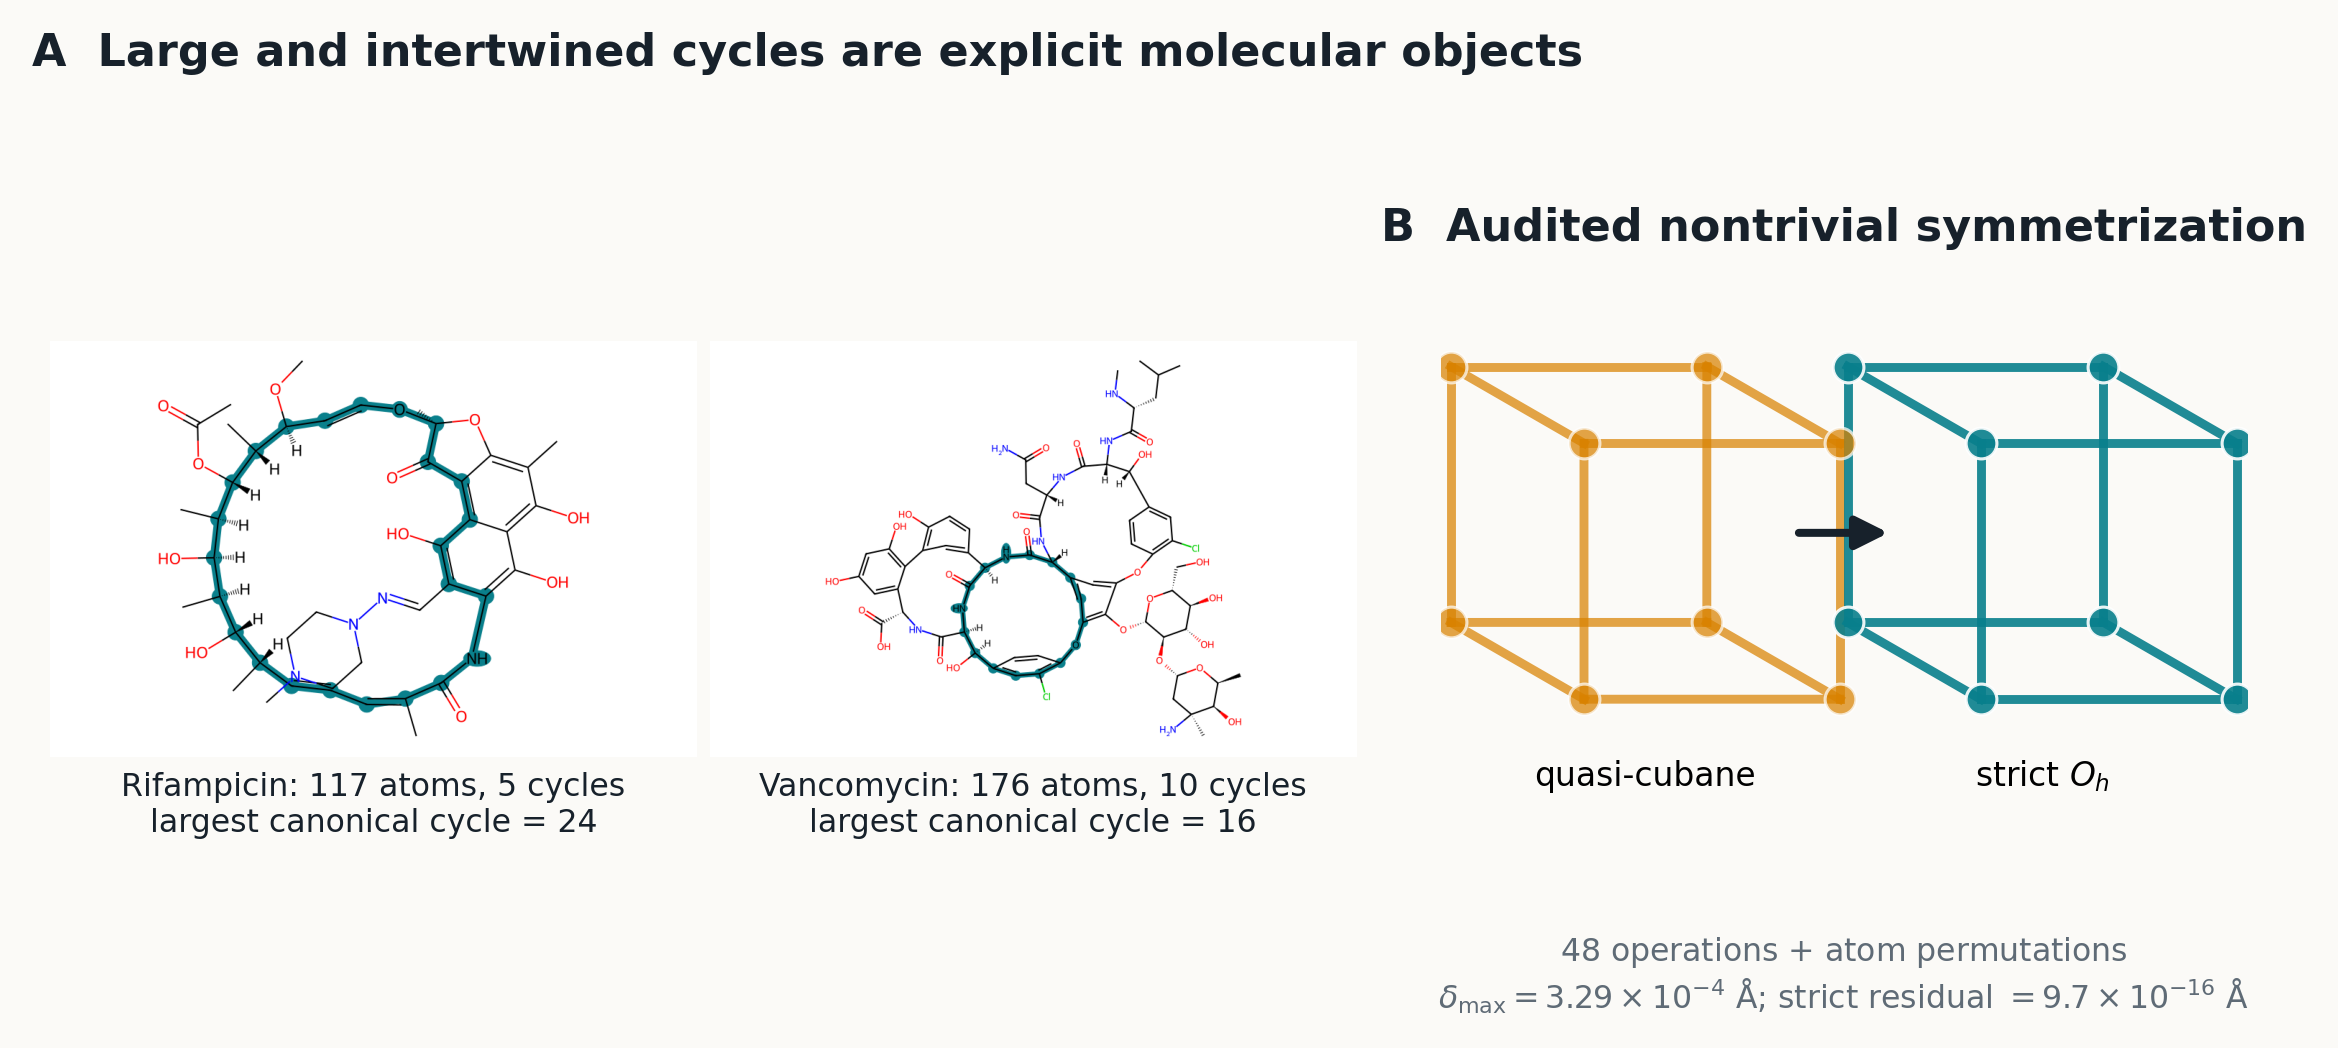
\includegraphics[width=\linewidth]{figures/oracle_chemical_scope.png}
\caption{Large-molecule perception and nontrivial symmetry. Panels (A)--(B) show intertwined cycles and the audited 48-operation $O_h$ symmetrization.}
\label{fig:large-systems}
\end{figure*}

All four cases recover a complete cycle basis and a Wilson rank of $3N-6$
(Figure~\ref{fig:large-systems}).  Rifampicin requires an ordered
24-membered ansa cycle within a five-cycle system, while vancomycin requires
ten canonical cycles, including two distinct 16-membered loops, in a
176-atom graph.  In each case the output is more than a ring count: it is an
executable ordered definition consumed by incidence, automorphism and
downstream coordinate constructors.

The second panel makes the parallel symmetry claim concrete.  Two vertices of
an analytic cubane were independently displaced before perception.  At the
declared $10^{-3}$~\AA\ tolerance, ORACLE recovers all 48 matrices and atom
permutations of $O_h$; group averaging moves any atom by at most
$3.29\times10^{-4}$~\AA, and strict reanalysis leaves a
$9.7\times10^{-16}$~\AA\ maximum residual.  The verified finite action
therefore controls the geometry-changing symmetrization.

Synthetic isolated cycles containing 16, 32, 64, 128, 256 and 512 vertices
each yield one complete rank-one cycle space.  This control demonstrates that
the production method retains the complete cycle independently of ring size.

\subsection{Test case III: hydrogen bonds add interaction resolution}

The water dimer is deliberately simple because it isolates a conceptual point.
From Cartesian coordinates alone, ORACLE identifies the covalent components
\{1,2,3\} and \{4,5,6\}, then perceives the interfragment
O1--H2$\cdots$O4 contact.  The 1.84~\AA\ H$\cdots$O distance,
$180^\circ$ angle and smooth weight 1.000 are stored separately from the
covalent edge set.  The same record generates an H2--O4 interaction primitive
coordinate.

The same molecular state therefore contains both the two covalent fragments
and the hydrogen-bonded assembly as coexisting resolutions.  For the calibrated
O--H$\cdots$O(H) class, a local model consumes the stored interaction
coordinate and produces a $+0.020$~\AA\ target.  This numerical response is
included to show how the persistent interaction object is reused: perception
establishes which interaction exists, whereas the application model decides
what quantity is calculated from it.  The reference domain and complete
parameters of that model are documented in the Supporting Information.

The same contract was then tested on intramolecular contacts of increasing
complexity (Figure~\ref{fig:perception-scope}).  Glycine I and II respectively
give zero and one accepted hydrogen bond, while retaining one and two weaker
interaction closures.  The C5 and C7 conformers of
N-acetylglycinamide---the glycine-dipeptide analogue---likewise distinguish a
weak C5 closure from the accepted N--H$\cdots$O contact of C7.\cite{puzzarini_glycine_dipeptide_2014}
The carbohydrate cases extend the test to oxygen-rich environments.  The symmetric \emph{c,c}
dihydroxyacetone conformer presents two donors to one acceptor; two
LCB26 $\alpha$-D-xylose conformers reverse the direction of their dominant
O--H$\cdots$O contact; and two D-fructose conformers contain three and four
accepted contacts within networks of nine and seven interaction closures.
For these compact systems, the CM5 reference can already contain one or more
intramolecular hydrogen bonds.  ORACLE therefore subtracts the tabulated
$s_c(\mathbf R_{\mathrm{ref}})\Delta\mathbf q_c$ contributions on the atoms
involved before storing $\mathbf q^0$; all later charge changes are generated
from this hydrogen-bond-free vector.  Thus the peptide and sugar examples
exercise the zero-contact and inverse-reference branches of the same
equations.
Every case retains a full-rank primitive set, while the individual contact
weights remain continuous---including a marginal 0.075 contact in the more crowded
fructose network---whereas acceptance, graph identity and primitive rank are
audited explicitly.  The result is stable chemical resolution throughout the
accepted connectivity basin.

\begin{figure*}[htbp]
\centering
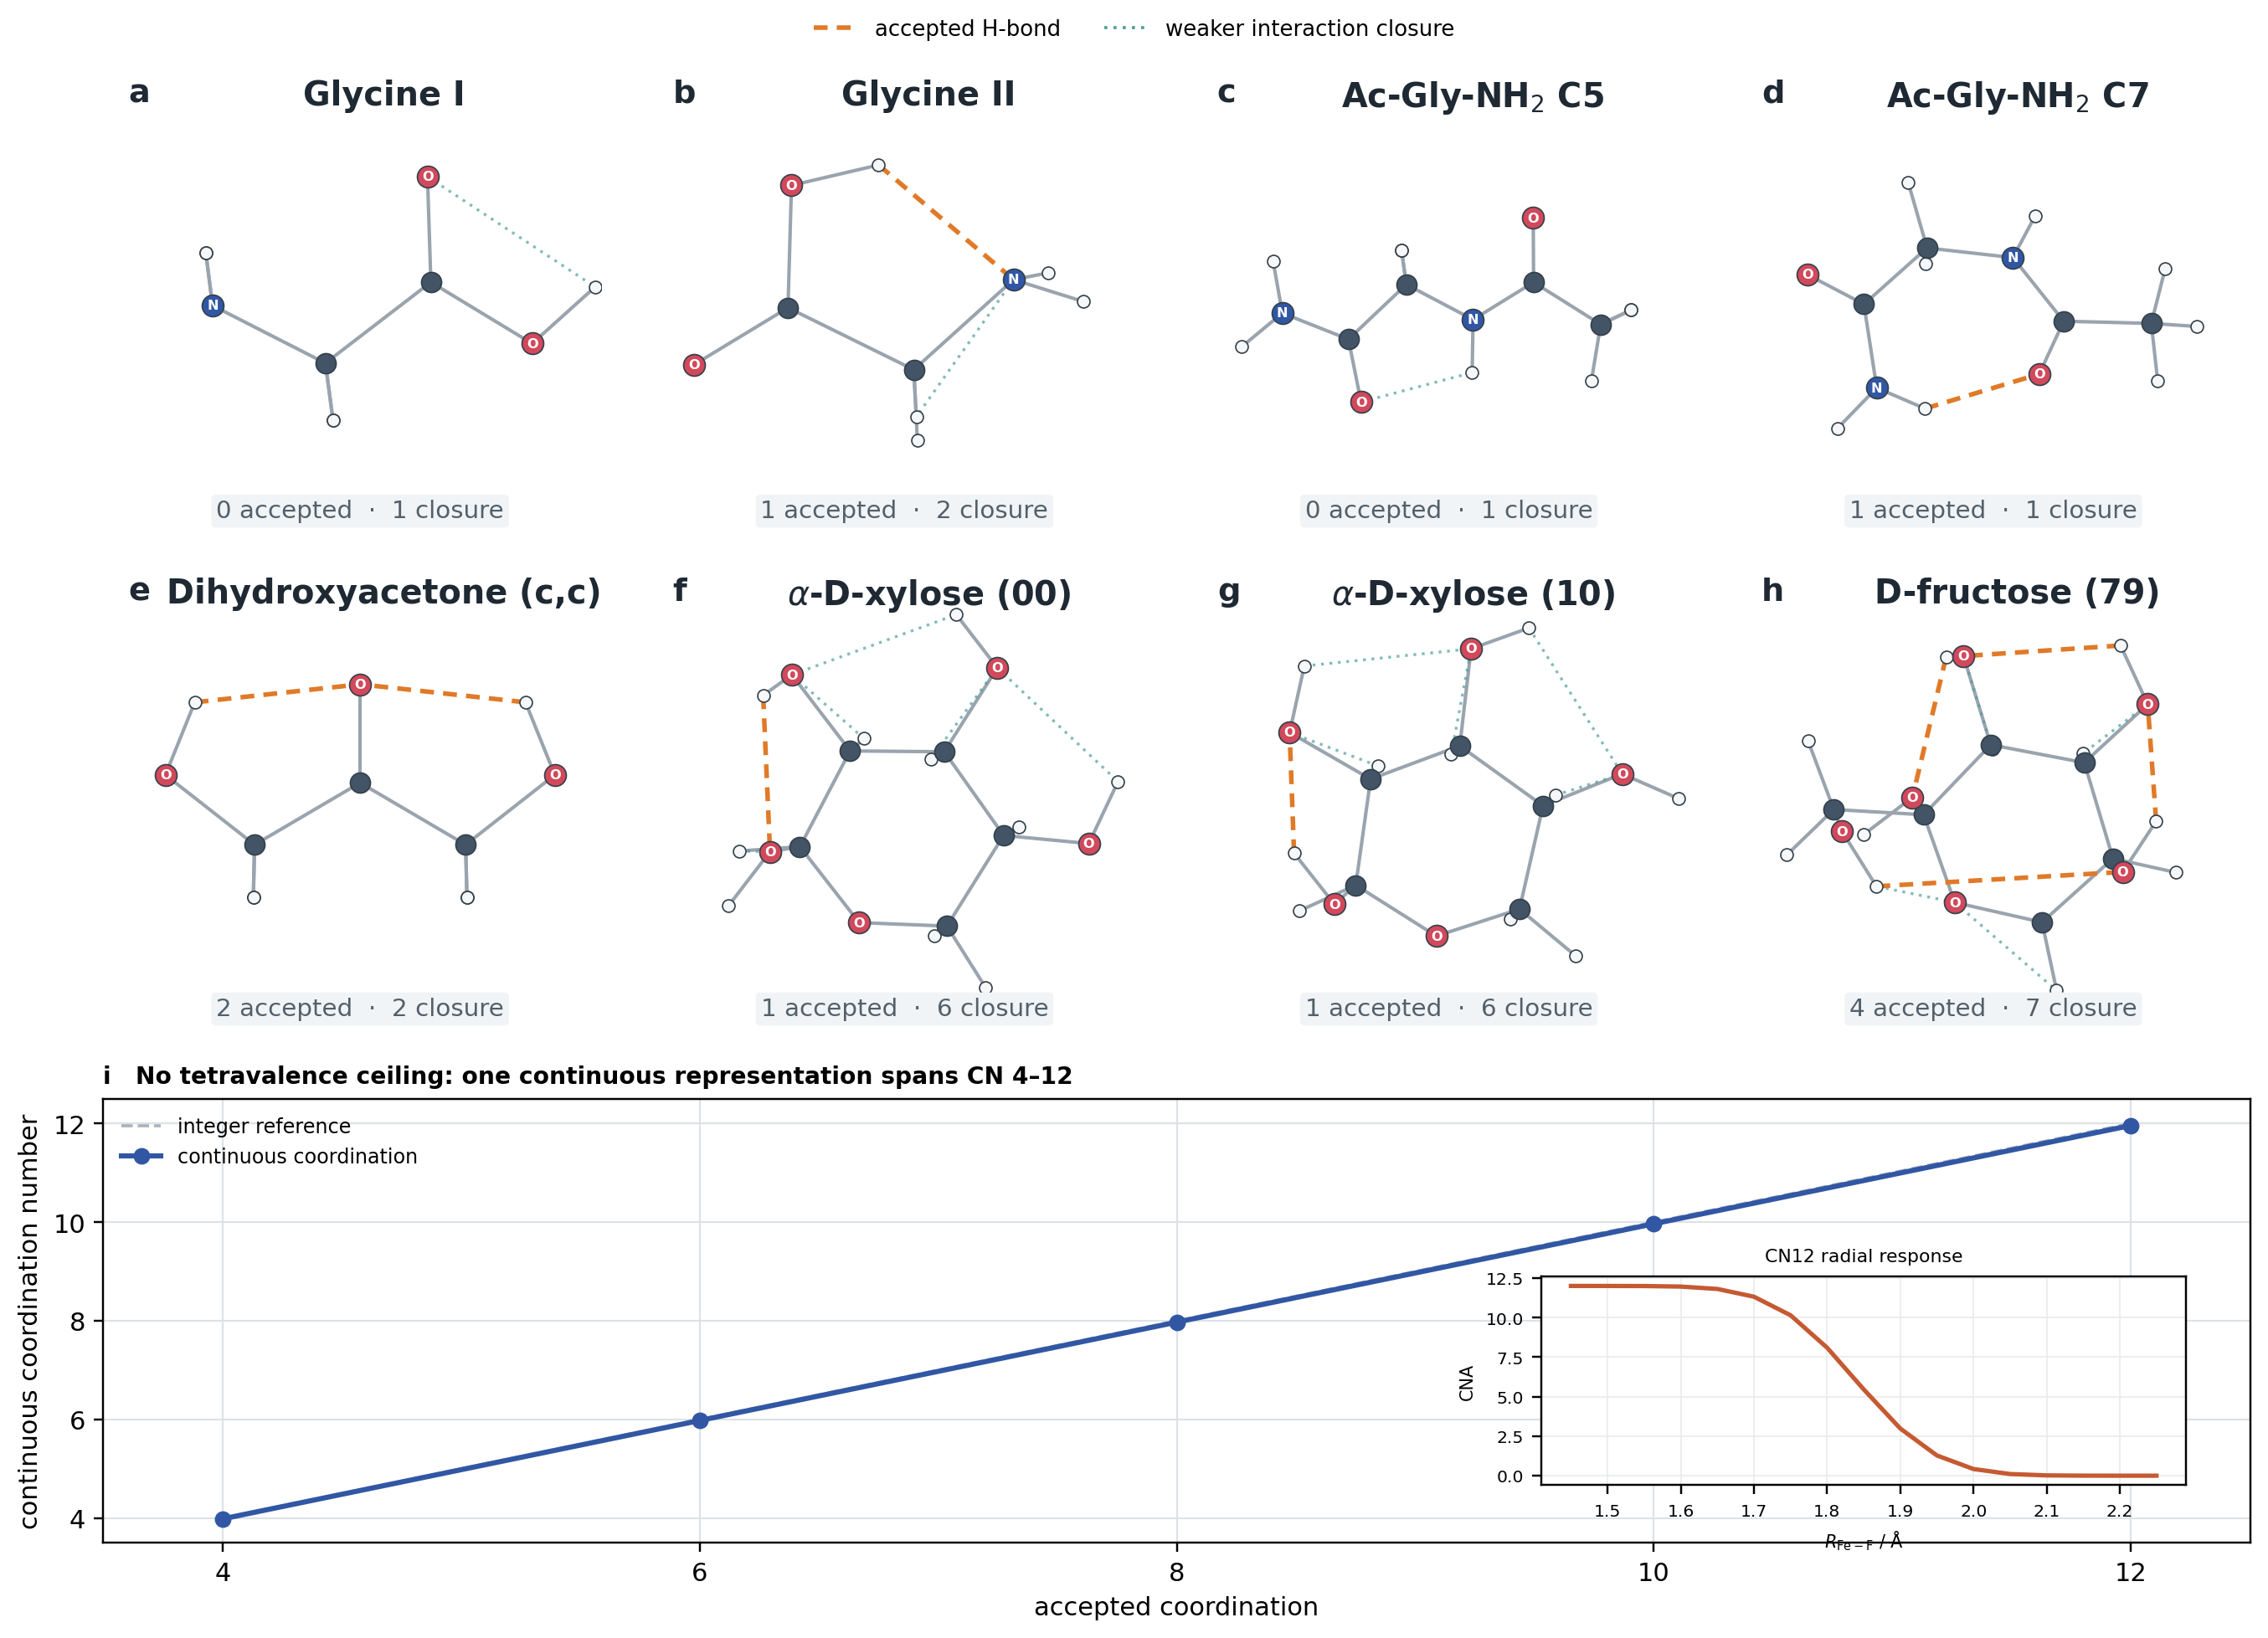
\includegraphics[width=\linewidth]{figures/oracle_perception_scope.png}
\caption{Continuous interaction and coordination evidence. Panels (a)--(h) show peptide-like and carbohydrate motifs; panel (i) spans coordination numbers 4--12.}
\label{fig:perception-scope}
\end{figure*}

\subsection{Test case IV: saccharin from perception to coverage diagnostics}

Saccharin couples a fused heterocycle, conjugation, polar sulfur bonds and
spectroscopic data in a compact 17-atom system.  Its geometry-only
electronegativity/Pauling observables correlate with the available Complete
Charge Model 5 charges and Mayer bond orders: Pearson/Spearman correlations
are 0.862/0.891 for charge and
0.907/0.924 for bond order.  Starting from the
equilibrium geometry, ORACLE identifies 18 transversal
core--valence targets
and 13 additional bond targets: six conjugated C--C and four C--H corrections,
together with two S--O and one S--N targets
examined here.  Equation~\ref{eq:backtransform} converges in two iterations
with a maximum residual of $8.6\times10^{-13}$.

The existing model leaves residuals of 3.148 and 3.471~m\AA\ for the S--O and
S--N environments.  The coordinate reconstruction remains successful, while
the coverage record distinguishes these sulfur environments from those
already represented.  The Supporting Information reports the sulfur
diagnostic and Hessian-threshold audit.
The corresponding structural audit is shown in Figure~\ref{fig:saccharin-structure}.

\begin{figure*}[htbp]
\centering
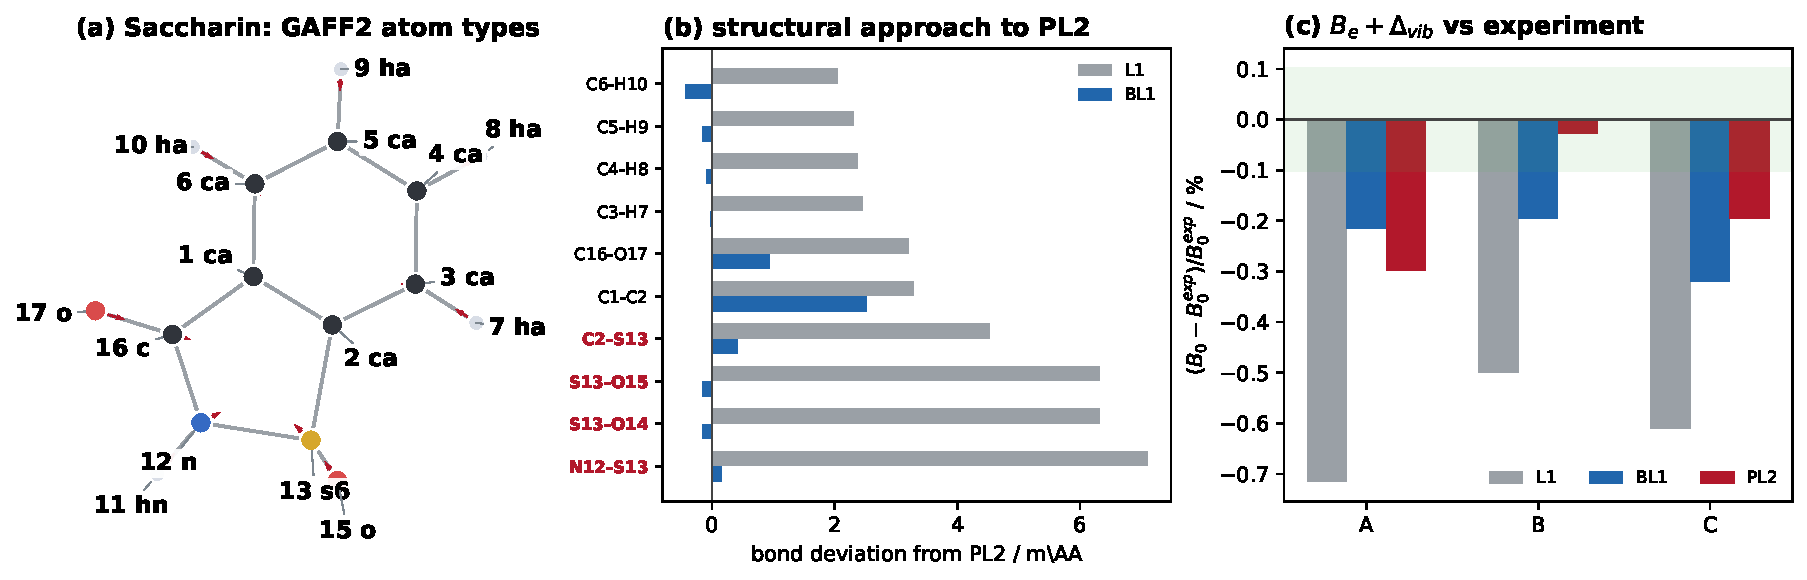
\includegraphics[width=\linewidth]{figures/oracle_saccharin_structure_case.pdf}
\caption{Saccharin structural audit and atom typing. Panels (a)--(c) show GAFF2 atom types, structural correction, and rotational constants versus experiment.}
\label{fig:saccharin-structure}
\end{figure*}

Transfer from a compact high-level library is precisely where a chemically
informed continuous representation should be most useful.  ORACLE perceives
all 331 structures at that reference level in the 2025 subset using the same
geometry-only information as the saccharin query, resolving whole-molecule
similarity into query-directed atom, bond and cycle coverage
(Figure~\ref{fig:retrieval}).

\begin{figure*}[htbp]
\centering
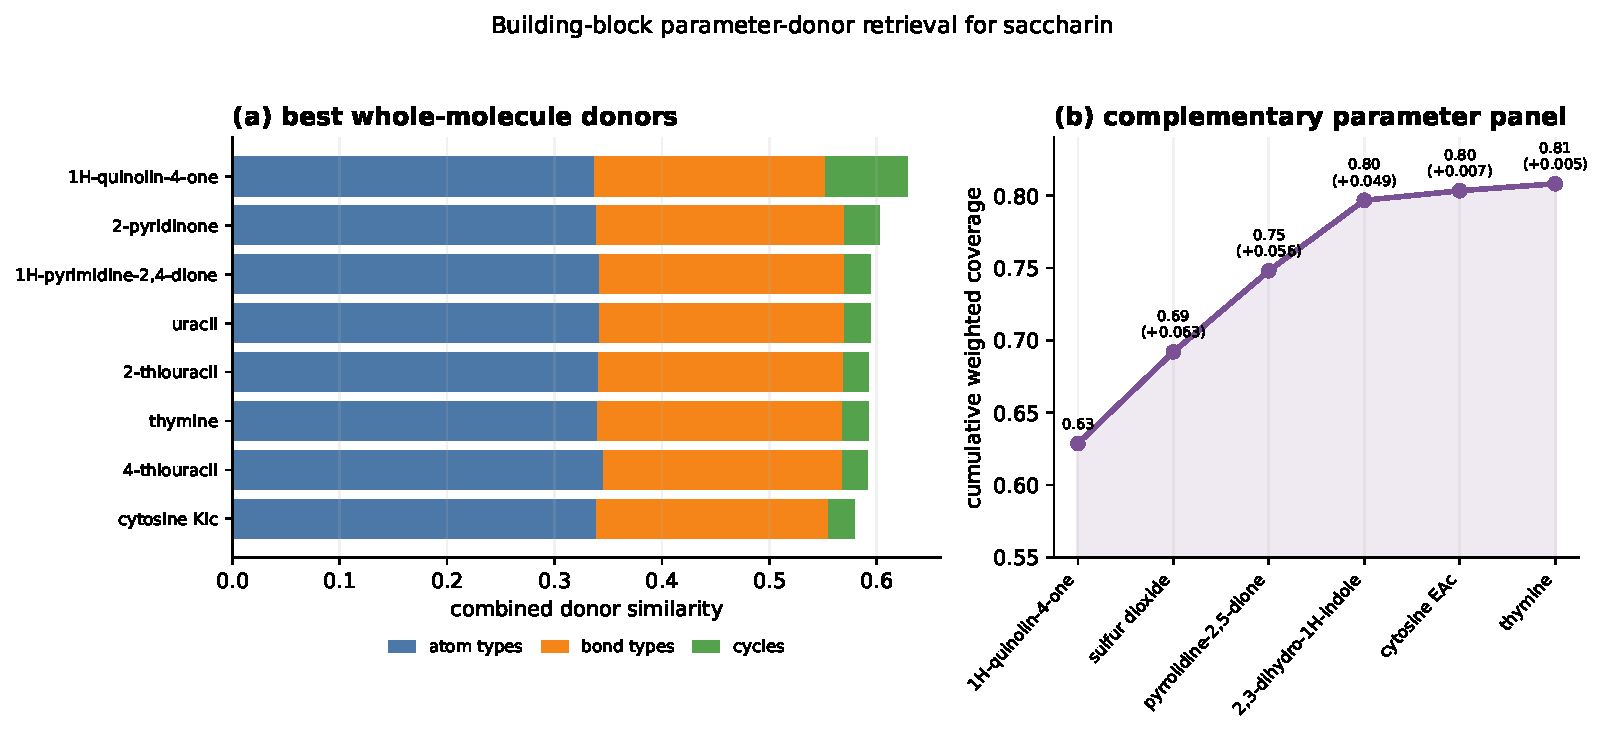
\includegraphics[width=\linewidth]{figures/oracle_saccharin_lcb25_retrieval.pdf}
\caption{Coverage-aware saccharin retrieval. Panels (a)--(b) show whole-molecule donors and the complementary parameter panel.}
\label{fig:retrieval}
\end{figure*}

The leading whole-molecule donor, 1H-quinolin-4-one, has combined similarity
0.629.  Adding complementary donors raises weighted coverage to 0.808
(Figure~\ref{fig:retrieval}); sulfur dioxide is selected early because it
supplies the best local S--O match despite being a poor global analogue.
The best S--N and C--S similarities remain approximately 0.001 or smaller.
The resulting coverage map identifies the distinct joint sulfur-centered
block and quantitatively rationalizes the inclusion of saccharin as the first
LCB26 member.

\subsection{Test case V: held-out local transfer}

A strict leave-one-out
control removes thiazole from the accurate reference pool, perceives its
independent lower-level input geometry, retrieves eight bond parameters from
other molecules and imposes them simultaneously through the ORACLE
primitive-coordinate back-transformation (Figure~\ref{fig:leave-one-out}).

\begin{figure*}[htbp]
\centering
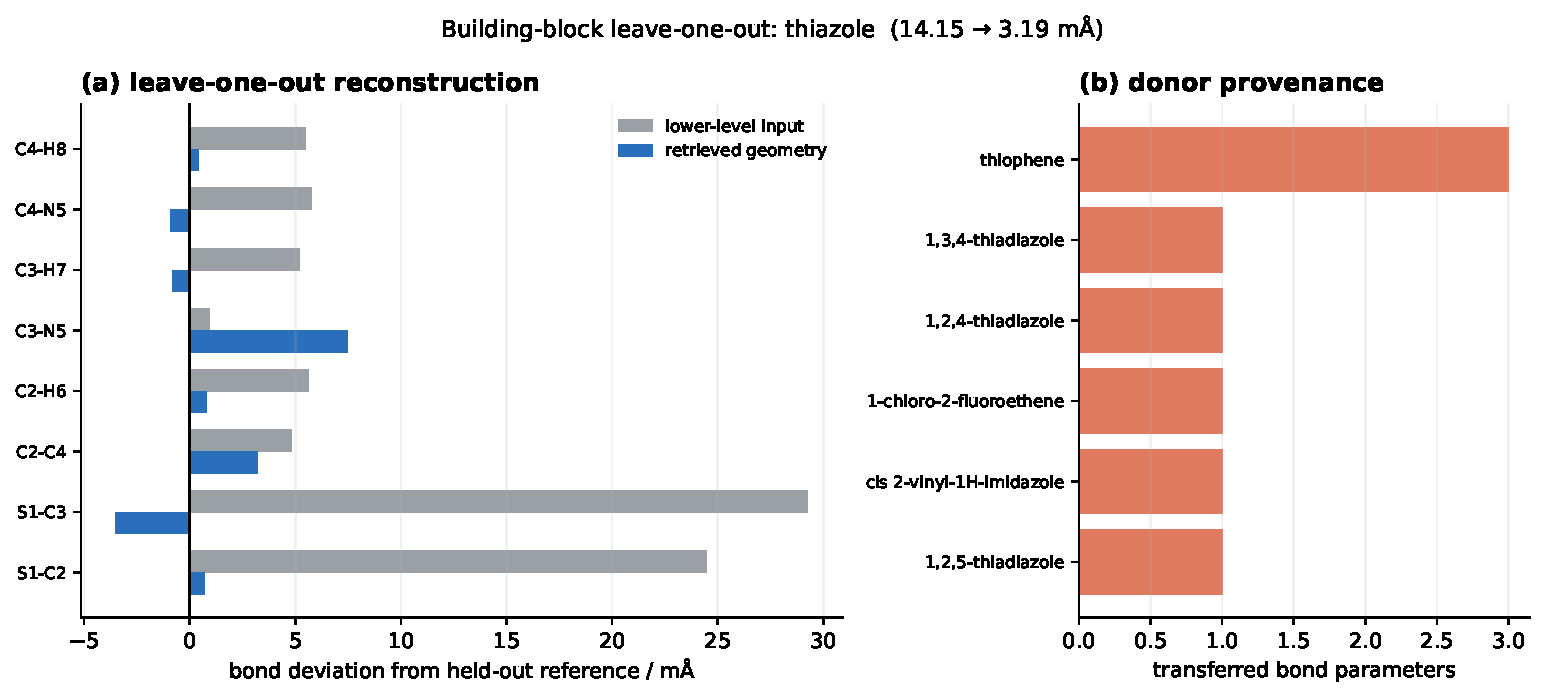
\includegraphics[width=\linewidth]{figures/oracle_lcb25_leave_one_out.pdf}
\caption{Held-out thiazole reconstruction. Panels (a)--(b) show the reconstruction and donor provenance.}
\label{fig:leave-one-out}
\end{figure*}

The retrieved donors have mean/minimum similarities 0.909/0.770.
Back-transformation converges in two iterations, reducing the bond RMS from
14.1 to 3.2~m\AA\ and the aligned Cartesian RMS from 14.5 to
5.1~m\AA\ (Figure~\ref{fig:leave-one-out}).  This predictive sparse-data
test shows that continuous perception can identify useful local donors, while
exact topology and primitive definitions ensure that transferred parameters act on
the intended molecular objects.
Seven targets satisfy the predeclared selector, and thiazole is the detailed
case shown here.  Together these seven leave-one-out reconstructions provide
a quantitative validation of local transfer under a frozen rule: donor
selection and reconstruction are completed before the accurate geometry of
each held-out target is used for scoring.

\subsection{Test case VI: from SMILES to a differentially corrected geometry}

The more demanding workflow begins from connectivity.  Thiazole is parsed and initialized by the same service,
relaxed with GFN-FF, and then optimized with the
second-generation Geometry, Frequency, Noncovalent extended tight-binding
method (GFN2-xTB) before being perceived once.  Its accurate reference entry
is reserved for final validation.  ORACLE identifies
34 required primitives---8 bonds, 11 angles, 12 dihedrals, and 3 out-of-plane
coordinates---selects ten distinct library donors, calculates those fragment
conformers with GFN2-xTB, and applies Equation~\ref{eq:differential}.  Explicit
donors support all 34 primitives (Figure~\ref{fig:xtb-differential}).

\begin{figure*}[htbp]
\centering
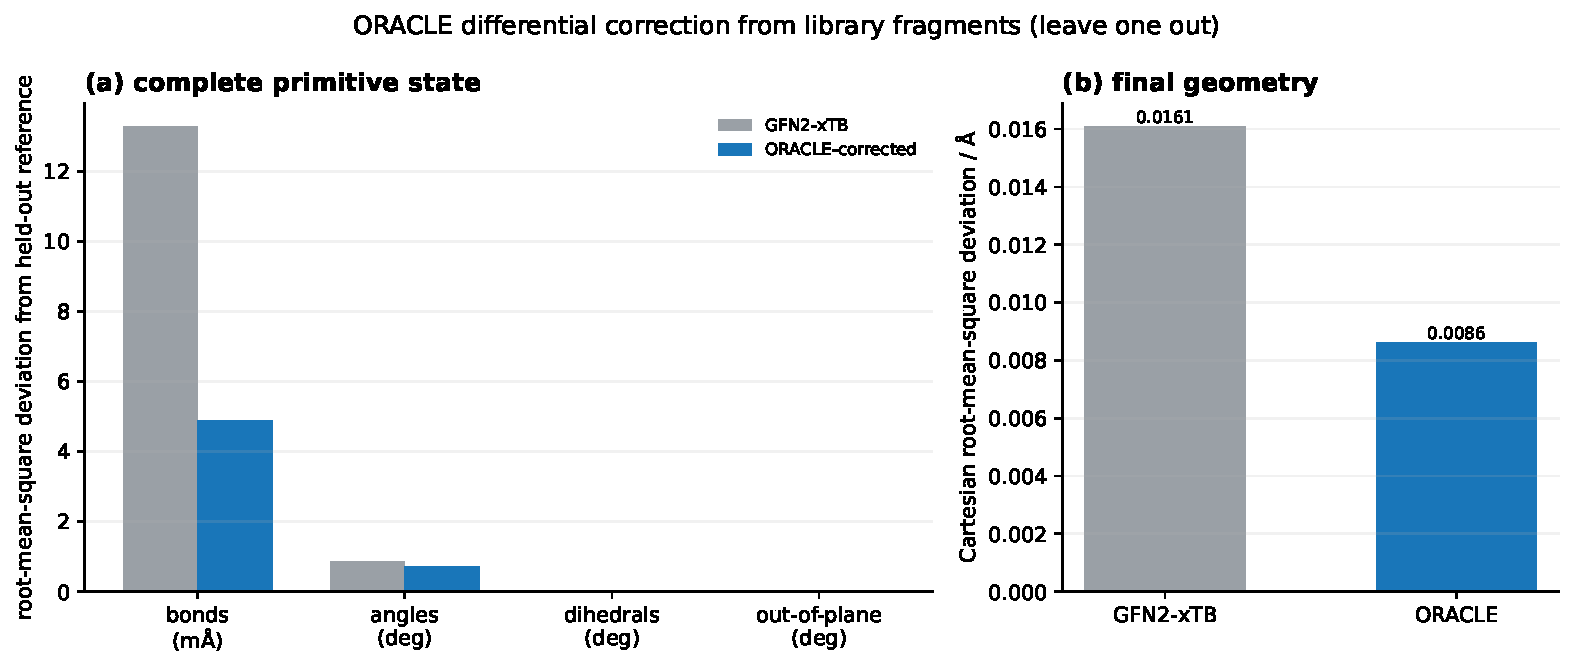
\includegraphics[width=\linewidth]{figures/oracle_lcb25_xtb_differential.pdf}
\caption{Held-out thiazole differential workflow. Panels (a)--(b) show the complete primitive state and final geometry.}
\label{fig:xtb-differential}
\end{figure*}

The bond RMS relative to the held-out accurate reference decreases from 13.3 to
4.9~m\AA, the angle RMS from 0.86 to 0.72$^\circ$, and the aligned
Cartesian RMS from 16.1 to 8.6~m\AA\
(Figure~\ref{fig:xtb-differential}).  ORACLE applies the 34 transfers
simultaneously and then uses the stored six-electron aromatic assignment and
$C_s$ action to apply the local-ring and finite-group projectors.  Dihedral
and out-of-plane RMS deviations remain below
$4\times10^{-7}$ degrees.  Persistence selects reference information and
constrains how that information may modify the molecule.

\section{A Common State for Molecular Workflows}

The practical implication is a change in workflow semantics.  A user no
longer passes an unexamined geometry from one application to the next; the
user passes a chemically typed state whose identity, evidence and invalidation
conditions travel with it.  This is particularly important when a medium-to-
large molecule is alternately optimized, fragmented, symmetrized, sampled and
reconstructed.  The state becomes the common scientific object, while files
and program calls become transport mechanisms.

For the user, the practical interface is simple: an organic SMILES
string or an enriched Cartesian/QCSchema record enters, and a consistent state within the supported chemical
domain emerges.  That state contains local descriptors and atom types, charges and bond
orders, rings, aromaticity, symmetry and fragments, together with constructed
or optimized structures when requested.  Fragment definition, charge
assignment and symmetrization therefore share one graph.

Continuity makes local environments stable under small geometric changes,
while exact rings and symmetry preserve the discrete objects required by
calculation.  Persistence records the thresholds and turns coverage into an
actionable quantity: within the H/C/N/O/F/P/S/Cl structural-library domain,
saccharin selects a sulfur-centered addition, while the carbohydrate subset
documents transfer across oxygen-rich environments.

Fragmentation closes the workflow in both directions.  ORACLE decomposes
large molecules into overlapping, charge-complete local objects and assembles
traceable structures from validated fragments.  Every assembled or optimized
geometry is re-perceived and audited against the same state.

\section{Conclusions}

ORACLE establishes a persistent chemical state in which molecular identity is
defined by continuous geometric and electronic evidence, accepted chemical
objects, and their explicit dependencies.  Atomic synthons and the effective
atomic number provide the central descriptors: they retain local chemical
meaning while remaining suitable for comparison, transfer and parameter
construction.  This creates a common representation for sophisticated
quantum-mechanical workflows on chemically important molecules in the
roughly 100--200 atom range.

The defining feature is the bidirectional exchange between perception and
quantum mechanics.  A single baseline calculation supplies charges, Mayer
bond orders and spin information that refine the chemical state; the refined
state then supports geometry generation, atom typing, force-field selection,
fragment assembly and subsequent electronic-structure calculations.  The
same mechanism distinguishes spin multiplicities, excited states, solvent
environments, transition states and high-coordination topologies at fixed or
changing geometries.

The validation demonstrates this scope through held-out structural transfer,
overlapping-fragment reconstruction, hydrogen-bond response, open-shell and
excited-state populations, reactive coordinate charts and polynuclear
coordination.  These applications share one persistent and inspectable state,
so chemical information remains available as a molecule moves between
representations and computational methods.  ORACLE therefore provides a
general foundation for efficient metrics, intelligent fragmentation,
solvent-aware and state-aware force fields, and reproducible integration of
advanced quantum chemistry across molecular science.

\section*{Data and Software Availability}

The data and software underlying this study are supplied in the Supporting
Information and in the public versioned repository
\url{https://github.com/yogibubu/ORACLE-standalone}.  The repository contains
the source, validation inputs, scripts and machine-readable records used here;
the ORACLE source is distributed under the BSD 3-Clause License.

\section*{Reproducibility}

The Supporting Information reports the complete theoretical definitions,
validation tables, input fingerprints, ordered ring sequences and exact
reproduction commands.  All reproduction scripts use portable relative paths.

\section*{Author Contributions}

Vincenzo Barone conceived the ORACLE methodology, developed the scientific
formulation and software, performed the validation, and wrote the manuscript.

\section*{Conflict of Interest}

The author declares no competing financial interest.

\begin{suppinfo}
Supporting Information includes the complete mathematical formulation,
parameter and notation definitions, structural-improvement models, topology
and aromaticity corpus, exact large-ring definitions, finite-group residuals,
quasi-symmetry threshold sweep, descriptor-invariance and atom-class audits,
symmetric-cubane projection, baseline charge and bond-order acquisition,
overlapping charge
synthesis, complete hydrogen-bond response vectors and fixed-geometry
metal-complex single points, compiled/Python backend equivalence,
saccharin and building-block-library numerical records, serialized-state tests
and exact
reproduction commands; auxiliary-code versions; Avogadro reimport semantics;
and the complete [6]helicene and carbohydrate overlap-assembly manifests,
coordinates and tests.
\end{suppinfo}

\clearpage
\bibliography{VB}

\begin{tocentry}
\centering
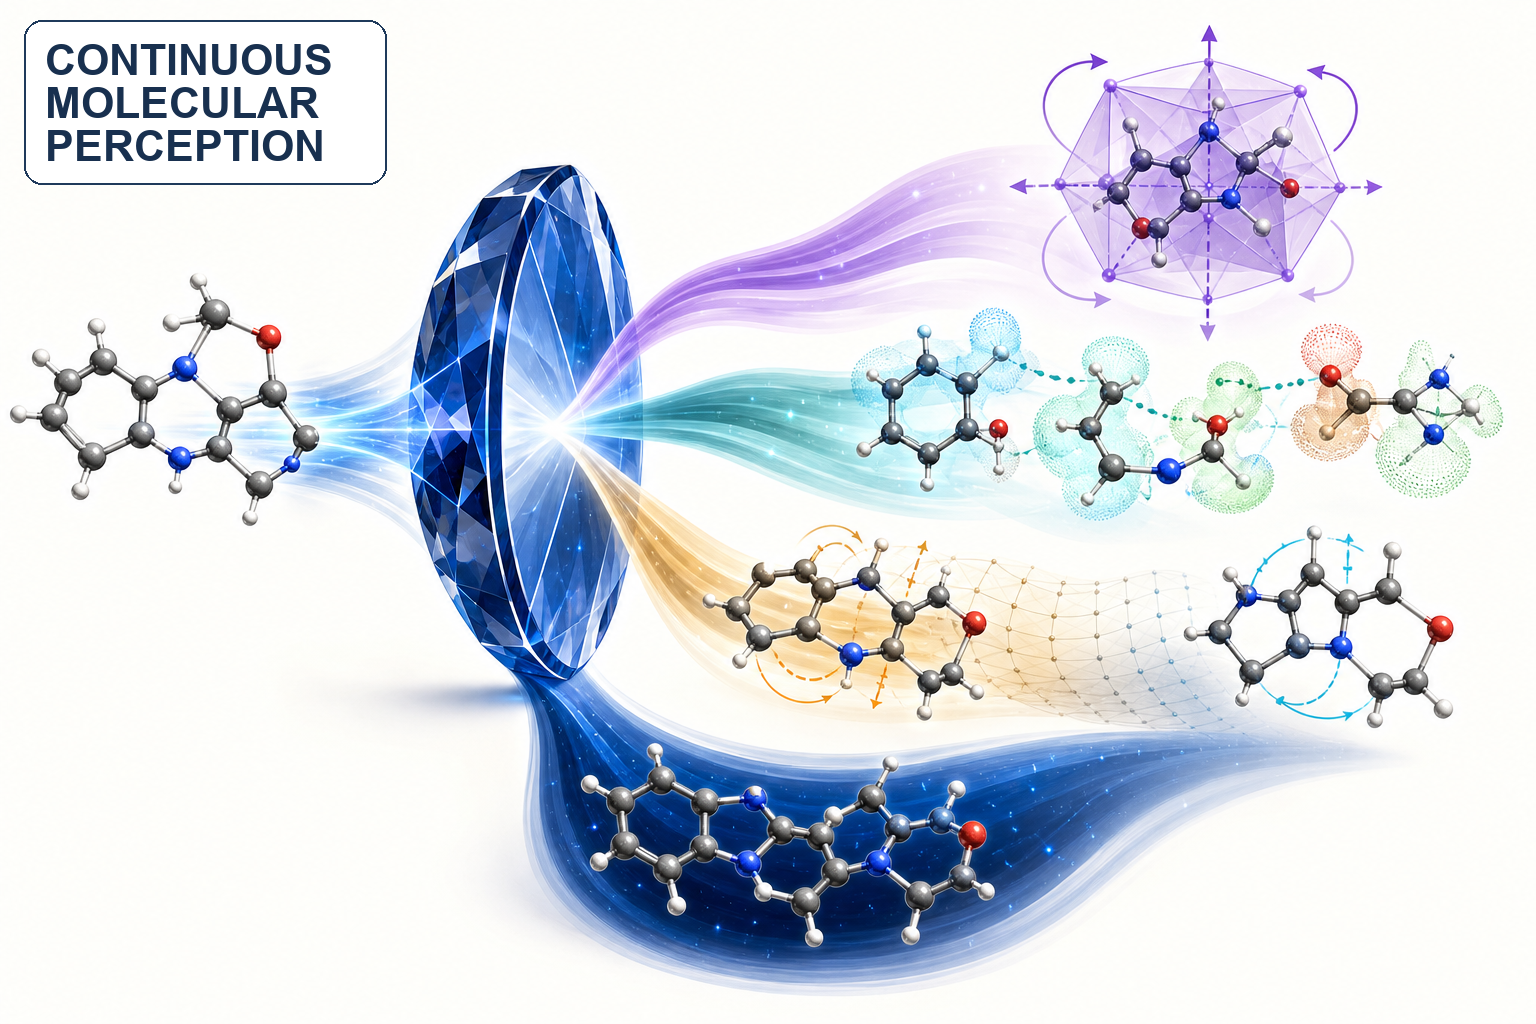
\includegraphics[height=4.35cm]{figures/oracle_toc_artistic_informative.png}
\end{tocentry}

\end{document}
